% Options for packages loaded elsewhere
\PassOptionsToPackage{unicode}{hyperref}
\PassOptionsToPackage{hyphens}{url}
\PassOptionsToPackage{dvipsnames,svgnames*,x11names*}{xcolor}
%
\documentclass[
  11pt,
  a4paper,
]{article}
\usepackage[]{mathpazo}
\usepackage{setspace}
\usepackage{amsmath}
\usepackage{ifxetex,ifluatex}
\ifnum 0\ifxetex 1\fi\ifluatex 1\fi=0 % if pdftex
  \usepackage[T1]{fontenc}
  \usepackage[utf8]{inputenc}
  \usepackage{textcomp} % provide euro and other symbols
  \usepackage{amssymb}
\else % if luatex or xetex
  \usepackage{unicode-math}
  \defaultfontfeatures{Scale=MatchLowercase}
  \defaultfontfeatures[\rmfamily]{Ligatures=TeX,Scale=1}
\fi
% Use upquote if available, for straight quotes in verbatim environments
\IfFileExists{upquote.sty}{\usepackage{upquote}}{}
\IfFileExists{microtype.sty}{% use microtype if available
  \usepackage[]{microtype}
  \UseMicrotypeSet[protrusion]{basicmath} % disable protrusion for tt fonts
}{}
\makeatletter
\@ifundefined{KOMAClassName}{% if non-KOMA class
  \IfFileExists{parskip.sty}{%
    \usepackage{parskip}
  }{% else
    \setlength{\parindent}{0pt}
    \setlength{\parskip}{6pt plus 2pt minus 1pt}}
}{% if KOMA class
  \KOMAoptions{parskip=half}}
\makeatother
\usepackage{xcolor}
\IfFileExists{xurl.sty}{\usepackage{xurl}}{} % add URL line breaks if available
\IfFileExists{bookmark.sty}{\usepackage{bookmark}}{\usepackage{hyperref}}
\hypersetup{
  pdftitle={Interannual climate variability mediates changes in carbon and nitrogen pools caused by annual grass invasion in a semi-arid shrubland},
  pdfauthor={Adam L. Mahood1,2 *; Rachel O. Jones3; David I. Board4; Jennifer K. Balch1,2; Jeanne C. Chambers4},
  colorlinks=true,
  linkcolor=RoyalBlue,
  filecolor=Maroon,
  citecolor=Blue,
  urlcolor=RoyalBlue,
  pdfcreator={LaTeX via pandoc}}
\urlstyle{same} % disable monospaced font for URLs
\usepackage[margin=1in]{geometry}
\usepackage{longtable,booktabs}
\usepackage{calc} % for calculating minipage widths
% Correct order of tables after \paragraph or \subparagraph
\usepackage{etoolbox}
\makeatletter
\patchcmd\longtable{\par}{\if@noskipsec\mbox{}\fi\par}{}{}
\makeatother
% Allow footnotes in longtable head/foot
\IfFileExists{footnotehyper.sty}{\usepackage{footnotehyper}}{\usepackage{footnote}}
\makesavenoteenv{longtable}
\usepackage{graphicx}
\makeatletter
\def\maxwidth{\ifdim\Gin@nat@width>\linewidth\linewidth\else\Gin@nat@width\fi}
\def\maxheight{\ifdim\Gin@nat@height>\textheight\textheight\else\Gin@nat@height\fi}
\makeatother
% Scale images if necessary, so that they will not overflow the page
% margins by default, and it is still possible to overwrite the defaults
% using explicit options in \includegraphics[width, height, ...]{}
\setkeys{Gin}{width=\maxwidth,height=\maxheight,keepaspectratio}
% Set default figure placement to htbp
\makeatletter
\def\fps@figure{htbp}
\makeatother
\setlength{\emergencystretch}{3em} % prevent overfull lines
\providecommand{\tightlist}{%
  \setlength{\itemsep}{0pt}\setlength{\parskip}{0pt}}
\setcounter{secnumdepth}{-\maxdimen} % remove section numbering
\pagestyle{plain}
\usepackage{lineno} % add 
\linenumbers % turns line numbering on 

% Allowing for landscape pages
\usepackage{lscape}
\newcommand{\blandscape}{\begin{landscape}}
\newcommand{\elandscape}{\end{landscape}}

% Left justification of the text: see https://www.sharelatex.com/learn/Text_alignment
% \usepackage[document]{ragged2e} % already in the latex template
\newcommand{\bleft}{\begin{flushleft}}
\newcommand{\eleft}{\end{flushleft}}
\usepackage{booktabs}
\usepackage{longtable}
\usepackage{array}
\usepackage{multirow}
\usepackage{wrapfig}
\usepackage{float}
\usepackage{colortbl}
\usepackage{pdflscape}
\usepackage{tabu}
\usepackage{threeparttable}
\usepackage{threeparttablex}
\usepackage[normalem]{ulem}
\usepackage{makecell}
\usepackage{xcolor}
\ifluatex
  \usepackage{selnolig}  % disable illegal ligatures
\fi
\newlength{\cslhangindent}
\setlength{\cslhangindent}{1.5em}
\newlength{\csllabelwidth}
\setlength{\csllabelwidth}{3em}
\newenvironment{CSLReferences}[2] % #1 hanging-ident, #2 entry spacing
 {% don't indent paragraphs
  \setlength{\parindent}{0pt}
  % turn on hanging indent if param 1 is 1
  \ifodd #1 \everypar{\setlength{\hangindent}{\cslhangindent}}\ignorespaces\fi
  % set entry spacing
  \ifnum #2 > 0
  \setlength{\parskip}{#2\baselineskip}
  \fi
 }%
 {}
\usepackage{calc}
\newcommand{\CSLBlock}[1]{#1\hfill\break}
\newcommand{\CSLLeftMargin}[1]{\parbox[t]{\csllabelwidth}{#1}}
\newcommand{\CSLRightInline}[1]{\parbox[t]{\linewidth - \csllabelwidth}{#1}\break}
\newcommand{\CSLIndent}[1]{\hspace{\cslhangindent}#1}

\title{Interannual climate variability mediates changes in carbon and nitrogen pools caused by annual grass invasion in a semi-arid shrubland}
\author{Adam L. Mahood\textsuperscript{1,2} * \and Rachel O. Jones\textsuperscript{3} \and David I. Board\textsuperscript{4} \and Jennifer K. Balch\textsuperscript{1,2} \and Jeanne C. Chambers\textsuperscript{4}}
\date{}

\begin{document}
\maketitle

\setstretch{2}
\small

\textsuperscript{1} Department of Geography, University of Colorado Boulder, Boulder, CO, USA

\textsuperscript{2} Earth Lab, University of Colorado, Boulder, CO, USA

\textsuperscript{3} Department of Biological \& Ecological Engineering, Oregon State University, Corvallis, Oregon, USA

\textsuperscript{4} US Forest Service, Rocky Mountain Research Station, Reno, NV, USA

\texttt{*} Corresponding author: \href{mailto:admahood@gmail.com}{\nolinkurl{admahood@gmail.com}}

\normalsize

\newpage

\hypertarget{abstract}{%
\section{ABSTRACT}\label{abstract}}

Exotic plant invasions alter ecosystem properties and threaten ecosystem functions globally. Interannual climate variability (ICV) influences both plant community composition (PCC) and soil properties, and interactions between ICV and PCC may influence nitrogen (N) and carbon (C) pools. We asked how ICV and non-native annual grass invasion covary to influence soil and plant N and C in a semiarid shrubland undergoing widespread ecosystem transformation due to invasions and altered fire regimes. We sampled four progressive stages of annual grass invasion at 20 sites across a large (25,000 km\(^2\)) landscape for plant community composition, plant tissue N and C, and soil total N and C in 2013 and 2016, which followed two years of dry and two years of wet conditions, respectively.

Multivariate analyses and ANOVAs showed that in invasion stages where native shrub and perennial grass and forb communities were replaced by annual grass-dominated communities, the ecosystem lost more soil N and C in wet years. Path analysis showed that high water availability led to higher herbaceous cover in all invasion stages. In stages with native shrubs and perennial grasses, higher perennial grass cover was associated with increased soil C and N, while in annual-dominated stages, higher annual grass cover was associated with losses of soil C and N. Also, soil total C and C:N ratios were more homogeneous in annual-dominated invasion stages as indicated by within-site standard deviations. Loss of native shrubs and perennial grasses and forbs coupled with annual grass invasion may lead to long-term declines in soil N and C and hamper restoration efforts. Restoration strategies that use innovative techniques and novel species to address increasing temperatures and ICV and emphasize maintaining plant community structure -- shrubs, grasses, and forbs -- will allow sagebrush ecosystems to maintain C sequestration, soil fertility and soil heterogeneity.

\emph{Keywords}: Annual grass conversion, soil carbon, soil nitrogen, soil homogenization, \emph{Bromus tectorum}, \emph{Artemisia tridentata}, path models, restoration

\newpage
\bleft

\hypertarget{introduction}{%
\section{1. INTRODUCTION}\label{introduction}}

Exotic plant invasions threaten biological diversity and ecosystem function (\protect\hyperlink{ref-Buckley2016}{Buckley \& Catford, 2016}; \protect\hyperlink{ref-Lonsdale1999}{Lonsdale, 1999}) and have long-term ecological consequences (\protect\hyperlink{ref-Mack2000}{Mack et al., 2000}). Plants modify the soil physical and chemical environment in ways that feed back to vegetation community composition and structure, and non-native, invasive plant species may alter soil properties in ways that differ from native plants (\protect\hyperlink{ref-DAntonio2009}{D'Antonio et al., 2009}; \protect\hyperlink{ref-Sardans2017}{Sardans et al., 2017}; \protect\hyperlink{ref-Schimel1991}{Schimel et al., 1991}; \protect\hyperlink{ref-Schimel1994}{Schimel et al., 1994}). In addition, there is increasing recognition that ``year effects'' have been generally overlooked in ecological studies (\protect\hyperlink{ref-Werner2020}{Werner et al., 2020}), and that interannual climatic variability can lead to boom and bust cycles where plant establishment, plant growth, and soil nutrient cycling are high in wet years and very low in dry years (\protect\hyperlink{ref-Hallett2019}{Hallett et al., 2019}; \protect\hyperlink{ref-Potts2019}{Potts et al., 2019}; \protect\hyperlink{ref-Puritty2019}{Puritty et al., 2019}). Understanding the differential effects of native and invasive plant species on soil and plant nitrogen (N) and carbon (C) and how these effects interact with interannual climatic variability may help explain the success of invasive species in water-limited environments (\protect\hyperlink{ref-Ehrenfeld2001}{Ehrenfeld et al., 2001}).

In the western United States, sagebrush (\emph{Artemisia} L. {[}Asteraceae{]}) ecosystems are being invaded by a non-native annual grass, \emph{Bromus tectorum} L. (Poaceae) (\protect\hyperlink{ref-Germino2016}{Germino et al., 2015}). In areas where native perennial grasses and forbs have been displaced, \emph{B. tectorum} can become the dominant understory component of the \emph{A. tridentata} community (\protect\hyperlink{ref-Chambers2007}{Chambers et al., 2007}; \protect\hyperlink{ref-Chambers2016}{Chambers et al., 2016}). This dominance can modify the pools and fluxes of soil C and N (\protect\hyperlink{ref-Hooker2008biogeochem}{Hooker et al., 2008}; \protect\hyperlink{ref-Leffler2016}{Leffler et al., 2016}), as well as increase fire probability by increasing the abundance and spatial continuity of fine fuels (\protect\hyperlink{ref-Bradley2018}{Bradley et al., 2018}; \protect\hyperlink{ref-Chambers2019}{Chambers et al., 2019}; \protect\hyperlink{ref-Davies2013}{Davies \& Nafus, 2013}). After a fire occurs, plant community composition often experiences several years of instability after which \emph{B. tectorum} can dominate (\protect\hyperlink{ref-Bradford2014}{Bradford et al., 2014}; \protect\hyperlink{ref-Davies2011}{Davies et al., 2011}; \protect\hyperlink{ref-Mack1981}{Mack, 1981}; \protect\hyperlink{ref-Mahood2019}{Mahood \& Balch, 2019}). Domination after a period of system instability implies a process of niche modification (\protect\hyperlink{ref-Fukami2015}{Fukami, 2015}; \protect\hyperlink{ref-Grman2010}{Grman \& Suding, 2010}) in which the invader alters the soil's physical and chemical environment in ways that facilitate its persistence (\protect\hyperlink{ref-DAntonio2009}{D'Antonio et al., 2009}; \protect\hyperlink{ref-Sardans2017}{Sardans et al., 2017}; \protect\hyperlink{ref-Schimel1991}{Schimel et al., 1991}; \protect\hyperlink{ref-Schimel1994}{Schimel et al., 1994}). This self-reinforcing feedback is also likely to be influenced by external drivers like climate (\protect\hyperlink{ref-Maestre2016}{Maestre et al., 2016}).

Interannual climatic variability is the primary control on soil water content in dryland systems (\protect\hyperlink{ref-Maestre2016}{Maestre et al., 2016}). Declines in the mean or large increases in the variability of water availability may lead to nonlinear top-down responses in ecosystem structure and function (\protect\hyperlink{ref-Belnap2016}{Belnap et al., 2016}; \protect\hyperlink{ref-McCluney2012}{McCluney et al., 2012}). These responses include increased invasion potential during periods when soil water content and nutrient availability exceed the uptake capacity of the native community (\protect\hyperlink{ref-Davis2000}{Davis et al., 2000}). Years with increased aridity can result in decreased concentrations of C and N due to reduced inputs from litter decomposition (\protect\hyperlink{ref-Crowther2016}{Crowther et al., 2016}; \protect\hyperlink{ref-Delgado-Baquerizo2013}{Delgado-Baquerizo et al., 2013}), lower biomass production and soil inputs (\protect\hyperlink{ref-Schwalm2010}{Schwalm et al., 2010}), and reduced cover of biological soil crusts (\protect\hyperlink{ref-Elbert2012}{Elbert et al., 2012}; \protect\hyperlink{ref-Ferrenberg2015}{Ferrenberg et al., 2015}; \protect\hyperlink{ref-Weber2016}{Weber et al., 2016}). Annual herbaceous plants are highly responsive to changes in temperature and moisture availability (\protect\hyperlink{ref-Bansal2016}{Bansal \& Sheley, 2016}; \protect\hyperlink{ref-Chambers2007}{Chambers et al., 2007}). This makes them well-suited to take advantage of episodic pulses of resource availability and their abundance can have profound effects on soil chemistry.

Soil nutrient cycling can differ between invaded and native ecosystems, in particular cycling of C and N (\protect\hyperlink{ref-Nagy2021}{Nagy et al., 2021}; \protect\hyperlink{ref-Wilsey2020}{Wilsey et al., 2020}). Many invasive species have high growth rates and nutrient concentrations that can result in increased rates of litter decomposition, mineralization, and nitrification (\protect\hyperlink{ref-Allison2005}{Allison \& Vitousek, 2005}; \protect\hyperlink{ref-Ehrenfeld2001}{Ehrenfeld et al., 2001}; \protect\hyperlink{ref-Liao2008}{Liao et al., 2008}; \protect\hyperlink{ref-Sardans2017}{Sardans et al., 2017}).

Additionally, soil texture interacts with precipitation to influence the rate of nutrient cycling and productivity (\protect\hyperlink{ref-Austin2004}{Austin et al., 2004}). Failing to account for soil texture when studying nutrient cycling could lead to spurious results. This is because in systems with annual precipitation below 370 mm, more soil water is lost via evaporation. Because water penetrates deeper into coarse-textured soils, they are more productive than finer textured soils due to lower soil water-holding capacity (the inverse texture hypothesis, \protect\hyperlink{ref-Noy-Meir1973}{Noy-Meir, 1973}; \protect\hyperlink{ref-Sala1988}{Sala et al., 1988}).

In \emph{A. tridentata} ecosystems, pools of inorganic and total N are often higher in \emph{B. tectorum}-invaded sites compared to uninvaded sites (\protect\hyperlink{ref-Booth2003}{Booth et al., 2003}; \protect\hyperlink{ref-Gasch2013}{Gasch et al., 2013}; \protect\hyperlink{ref-Hooker2008biogeochem}{Hooker et al., 2008}; \protect\hyperlink{ref-Johnson2011}{Johnson et al., 2011}; \protect\hyperlink{ref-Norton2004}{J. B. Norton et al., 2004}; \protect\hyperlink{ref-Stark2015}{Stark \& Norton, 2015}; but see \protect\hyperlink{ref-Rau2011}{Rau et al., 2011}). This is attributed to greater biomass turnover, faster rates of soil N cycling, and redistribution of inorganic N in surface soils (\protect\hyperlink{ref-Hooker2008biogeochem}{Hooker et al., 2008}). But single-year measurements of high N content are not necessarily indicative of long-term N storage, because the N cycle is highly sensitive to interannual climate variability (\protect\hyperlink{ref-Austin2004}{Austin et al., 2004}). In years with low, but highly variable soil moisture, the transformation of N by microbes and uptake of N by plants can be asynchronous. This is because microbes respond faster to smaller amounts of moisture than plants (\protect\hyperlink{ref-Dijkstra2012}{Dijkstra et al., 2012}). Furthermore, higher evaporation and soil temperatures in annual grass monocultures (\protect\hyperlink{ref-Turnbull2012}{Turnbull et al., 2012}) decreases the capacity of plants to activate and uptake labile N following small moisture pulses. Thus, inorganic N can accumulate in dry years due to production of inorganic N by microbes coupled with a lack of plant uptake (\protect\hyperlink{ref-Evans2001}{R. D. Evans et al., 2001}; \protect\hyperlink{ref-Hanan2017}{Hanan et al., 2017}; \protect\hyperlink{ref-Norton2008}{Norton et al., 2008}). This unused, labile N may leave the system via leaching or nitrification (\protect\hyperlink{ref-Austin2004}{Austin et al., 2004}; \protect\hyperlink{ref-Hanan2017}{Hanan et al., 2017}). When a system composed of deep-rooted perennial plants is converted to shallow-rooted herbaceous annuals, the depth that labile N must travel before it can no longer be accessed by the plant community decreases \protect\hyperlink{ref-Kulmatiski2020}{Kulmatiski et al.} (\protect\hyperlink{ref-Kulmatiski2020}{2020}).

In semi-arid shrubland systems of the western U.S., invasion by herbaceous species can interact with drought to reduce an ecosystem's capacity to sequester C (\protect\hyperlink{ref-Esch2019}{Esch et al., 2019}). \emph{A. tridentata} communities are a C sink during the growing season and this is amplified with increased summer precipitation (\protect\hyperlink{ref-Germino2016}{Germino et al., 2015}; \protect\hyperlink{ref-Huber2019}{Huber et al., 2019}). However, they may become a source with increases in dormant season precipitation (\protect\hyperlink{ref-Huber2019}{Huber et al., 2019}). While plants are dormant, the accelerated microbial C mineralization triggered by precipitation generates inorganic C that is susceptible to leaching or atmospheric losses via respiration (\protect\hyperlink{ref-Huber2019}{Huber et al., 2019}), without being offset by the C assimilation resulting from plant growth. \emph{A. tridentata} typically grows in neutral to slightly alkaline soils (\protect\hyperlink{ref-Hooker2008biogeochem}{Hooker et al., 2008}), and in alkaline soils some of the inorganic C may be composed of carbonates which can also be lost via leaching, only to accumulate at the bottom of hillslopes (\protect\hyperlink{ref-Johnson2014}{Johnson et al., 2014}). \emph{B. tectorum} monocultures sequester about half the C of sagebrush communities (\protect\hyperlink{ref-Germino2016}{Germino et al., 2015}), and can become a net source of C to the atmosphere with increasing summer drought (\protect\hyperlink{ref-Germino2016}{Germino et al., 2015}; \protect\hyperlink{ref-Prater2006}{Prater et al., 2006}). As with labile N, any labile C produced by episodic moisture pulses in the summer may be susceptible to leaching or atmospheric losses (\protect\hyperlink{ref-Norton2004}{J. B. Norton et al., 2004}).

In sagebrush shrublands, soil beneath shrubs and bunch grasses has higher total C and N than soil in shrub interspaces (\protect\hyperlink{ref-Bechtold2007}{Bechtold \& Inouye, 2007}; \protect\hyperlink{ref-Chambers2001}{Chambers, 2001}; \protect\hyperlink{ref-Ehrenfeld2005}{Ehrenfeld et al., 2005}; \protect\hyperlink{ref-Schlesinger1998}{Schlesinger \& M. Pilmanis, 1998}), and this may be altered with progressive invasion. Environmental heterogeneity creates niche diversity, which facilitates both invasion and coexistence between competitors via niche partitioning (\protect\hyperlink{ref-Lundholm2009}{Lundholm, 2009}; \protect\hyperlink{ref-Melbourne2007}{Melbourne et al., 2007}; \protect\hyperlink{ref-Shea2002}{Shea \& Chesson, 2002}; \protect\hyperlink{ref-Stein2014}{Stein et al., 2014}; \protect\hyperlink{ref-Tilman2004}{Tilman, 2004}). The loss of shrubs from fire and subsequent invasion of annual grasses yields a homogenous vegetation structure. The persistence of this simplified structure may lead to a more homogeneous distribution of soil nutrients. Soil nutrients are lost in the deeper layers and concentrated near the surface (\protect\hyperlink{ref-Nagy2021}{Nagy et al., 2021}), where they are being cycled by shallow, annual roots, and over time may become more evenly distributed rather than being concentrated around shrubs. In order to establish in such an environment, the roots of native seedlings must compete directly with annual grasses for water and nutrients in the near surface soil (\protect\hyperlink{ref-Cheng2004}{Cheng et al., 2004}), which is typically not as fully occupied by deep-rooted native perennials (\protect\hyperlink{ref-Gibbens2001}{Gibbens \& Lenz, 2001}).

Local variability in the abundance and chemical composition of plants may mediate the effect of climatic forces, but the idiosyncratic ways in which species respond to environmental change is not always linearly related to the effect they have on ecosystem processes (\protect\hyperlink{ref-Felton2018}{Felton et al., 2018}; \protect\hyperlink{ref-Suding2008}{Suding et al., 2008}). Climatic conditions affect plant tissue C:N ratios, which influence flammability, decomposition rates (\protect\hyperlink{ref-Grootemaat2015}{Grootemaat et al., 2015}) and soil inputs of C and N (\protect\hyperlink{ref-Norton2004}{J. B. Norton et al., 2004}). In dry years, plants may allocate resources towards root or seed production at the expense of above-ground growth (\protect\hyperlink{ref-Franklin2016}{Franklin et al., 2016}; \protect\hyperlink{ref-Grime1977}{Grime, 1977}). This leads to higher quality litter (lower C:N), which allows for faster N cycling in the ensuing years. In wet years more above-ground growth may lead to higher C:N ratios, lower quality litter, and slower N cycling in the ensuing years. However, the relative abundance of forbs to grasses increases with growing season precipitation (\protect\hyperlink{ref-Felton2018}{Felton et al., 2018}; \protect\hyperlink{ref-Hallett2019}{Hallett et al., 2019}). This increases litter quality and decomposition rates because forbs have higher leaf N content (\protect\hyperlink{ref-Cornwell2008}{Cornwell et al., 2008}). Thus, while increased water availability may increase plant C:N ratios by species, the increased abundance of forbs may cause a decrease in community mean C:N ratios. The resulting lagged effect of climate on litter quality (\protect\hyperlink{ref-Evans2001}{R. D. Evans et al., 2001}; \protect\hyperlink{ref-Pilliod2017}{Pilliod et al., 2017}) feeds back to soil C and N cycles (\protect\hyperlink{ref-Yelenik2010}{Yelenik \& Levine, 2010}).

This broad-scale, observational study was designed to evaluate how progressive stages of \emph{B. tectorum} invasion alter soil and plant nutrients in \emph{A. tridentata} ssp. wyomingensis ecosystems in the context of interannual climatic variability. In previous studies examining the mechanisms by which \emph{B. tectorum} influences soil nutrient cycling, soil samples were typically collected from vegetation patches within single sites that were either invaded or not invaded by \emph{B. tectorum} (\protect\hyperlink{ref-Blank2008}{Blank, 2008}; \protect\hyperlink{ref-Evans2001}{R. D. Evans et al., 2001}; \protect\hyperlink{ref-Rimer2006}{Rimer \& Evans, 2006}; \protect\hyperlink{ref-Sperry2006}{Sperry et al., 2006}). Studies that sampled several locations (\protect\hyperlink{ref-Norton2004}{J. B. Norton et al., 2004}) included a range of soil types. The only climatic context given was usually 30 year normals. To our knowledge, no published studies have examined how progressive \emph{B. tectorum} invasion influences soil and plant C and nutrients at the plant community or landscape scale. To evaluate how invasion and interannual climate variability affect soil and plant C and N, we examined four progressive stages of invasion. We sampled soil, litter and plant tissue in 2013, which followed two years of dry conditions, and in 2016, which followed two years of wet conditions. We had three hypotheses: (1) Loss of \emph{Artemisia} shrubs and increases in \emph{B. tectorum} cover reduces soil total C and N pools and homogenizes soil total C and N and other soil nutrients. (2) Higher water availability results in increased plant cover, greater plant tissue C:N ratios, and decreased soil total N, total C, and C:N ratios. (3) The primary drivers of soil and plant C and N differ for invasion stages with \emph{Artemisia} shrubs and those dominated by \emph{B. tectorum}.

\hypertarget{methods}{%
\section{2. METHODS}\label{methods}}

\hypertarget{study-area}{%
\subsection{2.1 Study Area}\label{study-area}}

The study area encompassed 25,000 km\(^2\) Northern and Central Basin and Range Ecoregions (hereafter, Great Basin), in the north-central part of the state of Nevada in the western U.S. Twenty sites with the same soil type were selected for study after reviewing Bureau of Land Management (BLM) fire and soil maps and consulting with land managers from the BLM Winnemucca Field Office. All sites had similar slopes (0-5\%) and elevations (1297-1607 m) and were located at least 1.5 km apart to ensure statistical independence. Mean temperatures ranged from 19°C in July to -1°C in January. Precipitation ranged from 254-304 mm with most arriving as snow in fall and winter. All sites had similar soil textures and minimal, if any carbonate content (Table S1) (\protect\hyperlink{ref-OGeen2017}{O'Geen et al., 2017}), and represented the same ecological site type: Loamy 10-12 precipitation zone/ \emph{A. tridentata} ssp. \emph{wyomingensis} (Wyoming big sagebrush) and \emph{Achnatherum thurberianum} (Piper) Barkworth (Poaceae, Thurber's needlegrass). All sites had the same grazing regime, which was grazing from summer through fall. The grazing allotments where our study sites were located were allotted an average 10 \(\pm\) 6 billed animal unit months per square kilometer. In other words, 1 cow with her calf, or 5 sheep plus their lambs, for 10 months per square kilometer (\protect\hyperlink{ref-NRCS2003}{NRCS, 2003}).

The sites had four stages of \emph{B. tectorum} invasion: (1) six sites with a mature sagebrush canopy, 0-5\% aerial cover of \emph{B. tectorum}, and no fires within the last 30 years (I. intact sagebrush), (2) five sagebrush sites with 5-20\% \emph{B. tectorum} cover and no recent fires (II. invaded sagebrush), (3) five cheatgrass-dominated sites with recent (\textless{} 5 years before 2013) fires (III. cheatgrass-dominated), and (4) four cheatgrass die-off sites, where \emph{B. tectorum} failed to emerge, establish, or reproduce in areas that supported dense \emph{B. tectorum} stands in previous years (\protect\hyperlink{ref-Baughman2013}{Baughman \& Meyer, 2013}) (IV. cheatgrass die-off). These later sites were a year or two post-die-off in 2013, had some \emph{B. tectorum} plants (\textasciitilde{} 5\% cover), and were generally dominated by nonnative annual forbs such as \emph{Erodium cicutarium} (L.) L'Hér. ex Aiton (Geraniaceae), \emph{Sisymbrium altissimum} L. (Brassicaceae) and \emph{Lepidium perfoliatum} L. (Brassicaceae). Five sites (3 cheatgrass-dominated, 2 intact sagebrush) that were sampled in 2013 were not re-sampled in 2016 due to access issues.

\hypertarget{field-data-collection}{%
\subsection{2.2 Field data collection}\label{field-data-collection}}

At each site, we established six, 50 m transects that were parallel and spaced 20 m apart. Transects were measured in adjacent pairs, yielding 3 replicates per site. We measured shrub cover and collected composite samples of soils and litter biomass along these transect pairs before active growth began in early-mid April 2013 and in late March 2016. The transect pairs were re-sampled during peak production in early-mid June 2013 and in mid-late June 2016. During the second visit, we estimated the cover of all plant species and ground cover and collected composite samples of herbaceous vegetation for nutrient analysis. A list of all species encountered is in the supplementary material (Table S2)

We measured the cover of all shrub species at each site using the line-intercept method in 2013 (\protect\hyperlink{ref-Elzinga1998}{Elzinga et al., 1998}). The length of each shrub that intercepted the transect line was measured and then the lengths were summed to calculate total shrub distance. Percent shrub cover was determined by dividing the total shrub distance by the total transect distance.

In April 2013 and March 2016, litter and soil samples were collected systematically every 5m along each transect for a total of 11 samples per transect (n = 22 per transect pair, n = 66 per site). Litter biomass was removed from a 15x15 cm patch at each sampling location along the transect, and then soil samples were collected from the same locations with a punch auger to a depth of 0-10 cm. Soil samples from each transect pair were placed in a bucket and homogenized, returned to the lab, and sieved to \textless2 mm. Soil samples (n = 3 sub-samples per site) were air-dried and sent to the Soil, Water and Forage Analytical Laboratory (SWFAL) at Oklahoma State University where they were analyzed for percent total C and total N using a LECO TruSpec CN Analyzer (LECO Corp., St.~Joseph, MI, USA), and NO\(_3\) -N and NH\(_4\) -N using KCl extraction and quantification with a Lachat® autoanalyzer. Soil Mg and Ca were measured using Mehlich 3 extraction and quantification with a Spectro ICP, and SO\(_4\) -S using calcium phosphate monobasic extraction and quantification with a Spectro ICP. One bulk density sample was collected systematically at each transect pair, for a total of three samples per plot, with a 6 cm tall x 5 cm diameter metal cylinder. Samples were returned to the lab, dried at 105 degrees Celsius and weighed after the mass stabilized. Samples were then sieved to \textless2 mm. The weight and volume of any gravel removed was subtracted from the raw bulk density measurements. We used the mean of the three adjusted bulk density measurements at each plot to convert concentrations measured in the lab to area-based content. Litter biomass was oven dried at 60° C, ground in a Udy mill, and then sent to SWFAL where it was analyzed for total C and N using a LECO TruSpec CN Analyzer (LECO Corp., St.~Joseph, MI, USA).

In June, a 0.1m2 quadrat was placed along the transect adjacent to the litter and soil sampling location and used to visually estimate basal and aerial cover of all species, litter, bare ground, rocks, cryptograms, and dung. Standard protocols were used and frequent calibrations among estimators were conducted (\protect\hyperlink{ref-Elzinga1998}{Elzinga et al., 1998}). We used these estimates to summarize species cover by functional groups: native shrubs (SH), perennial native grasses (PNG), perennial native forbs (PNF), annual native forbs (ANF), annual invasive grasses (AIG), and annual invasive forbs (AIF). After cover was estimated, aboveground biomass of \emph{B. tectorum}, \emph{Poa secunda} J. Presl (Poaceae), and all other herbaceous plants were harvested from the same quadrats. Samples were homogenized for the three different categories for every transect pair (n = 3 sub-samples per site) as was done for litter and soils. If either \emph{B. tectorum} or \emph{P. secunda} were not collected from within the quadrats, an additional sample was taken nearby from within the site. Homogenized vegetation sub-samples were returned to the lab where they were oven dried at 60°C, ground, and weighed. Vegetation sub-samples were then sent to SWFAL for analysis of total C and N using a LECO TruSpec CN Analyzer (LECO Corp., St.~Joseph, MI, USA).

\hypertarget{climate-data}{%
\subsection{2.3 Climate data}\label{climate-data}}

We used minimum temperature (T\(_\text{min}\)), actual evapotranspiration (AET), precipitation, and climatic water deficit (CWD) derived from gridMET (\protect\hyperlink{ref-Abatzoglou2013}{Abatzoglou, 2013}) (Figure 1) to evaluate how climatic variability interacted with plant-soil relationships. We chose these variables because they closely reflect physical conditions important for plant growth and survival. Minimum temperature is important because of the effects of freezing, while AET and CWD represent the supply and demand components of atmospheric water balance (\protect\hyperlink{ref-Dobrowski2013}{Dobrowski et al., 2013}). We calculated precipitation for the water year preceding sampling because of the effects of antecedent precipitation on annual grass biomass and cover (\protect\hyperlink{ref-Pilliod2017}{Pilliod et al., 2017}).

\begin{figure}
\centering
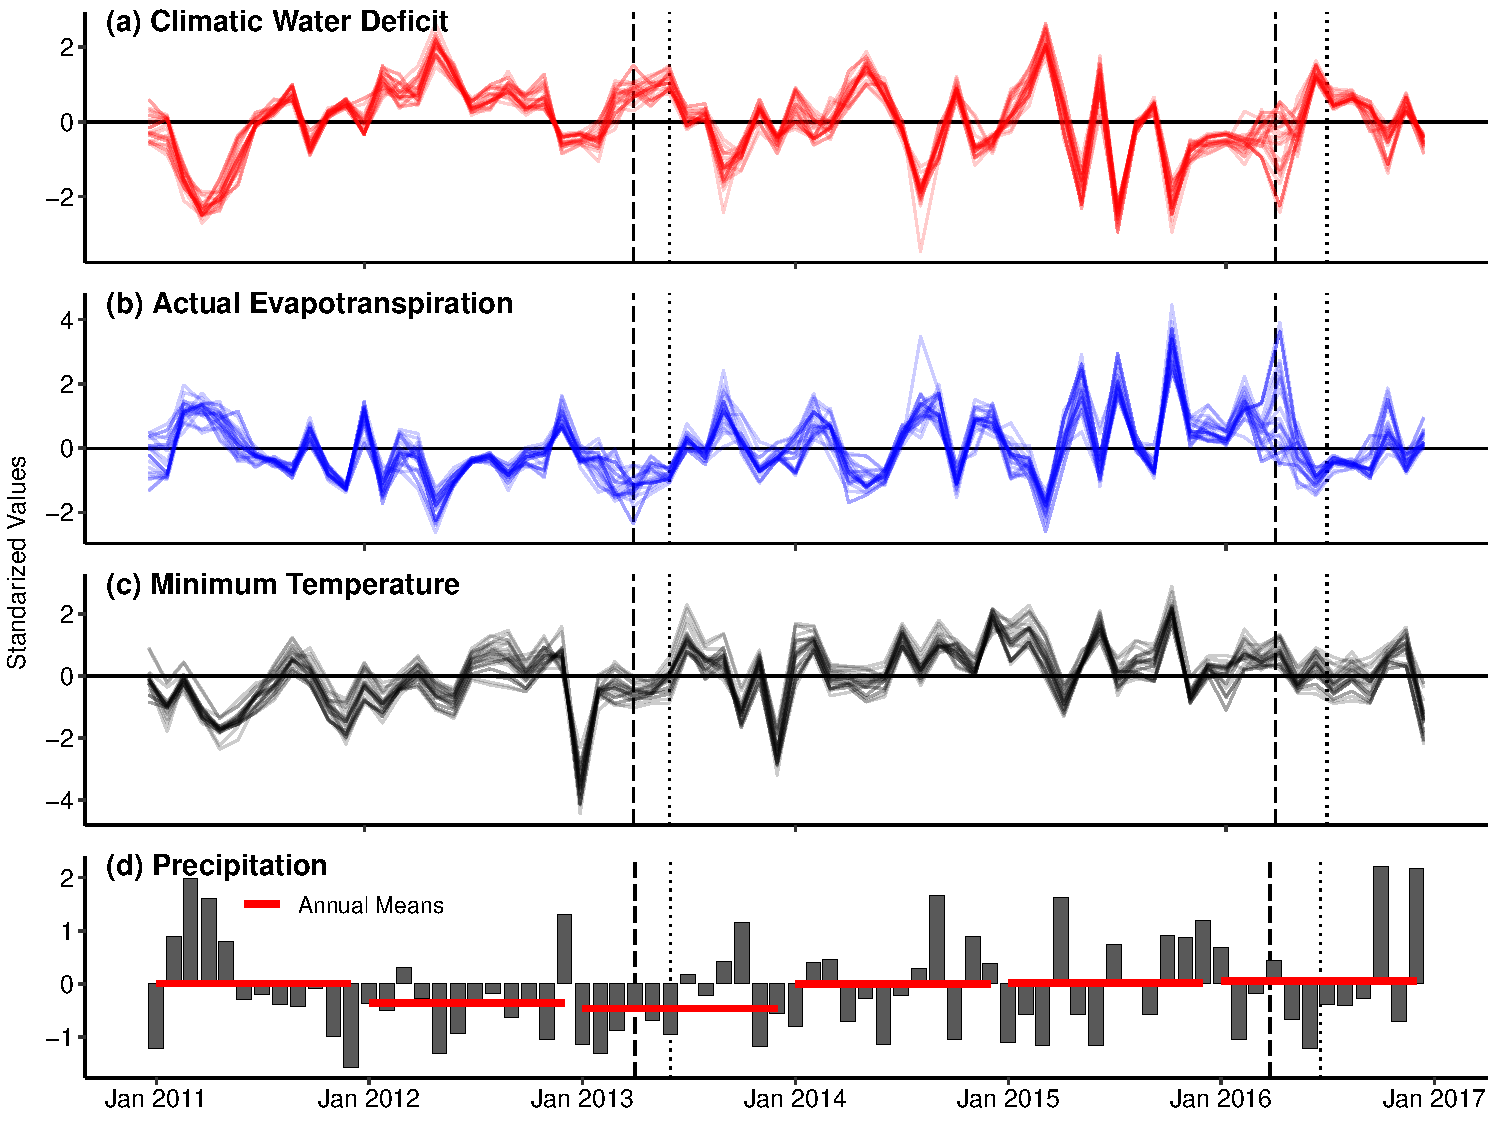
\includegraphics{figures/figure_1_climate.pdf}
\caption{Climatic conditions from January 2011 to January 2017 at the study sites. Dashed vertical lines are the dates of soil and litter sampling, dotted vertical lines are the dates of vegetation cover and biomass sampling. a-c show the monthly anomaly from 30-year normals of actual evapotranspiration, climatic water deficit, and minimum temperature, with each line representing one study site. In d, bars show the monthly precipitation anomaly at the Winnemucca, Nevada airport. The red lines represent yearly averages.}
\end{figure}

\hypertarget{analyzing-changes-in-community-composition}{%
\subsection{2.4 Analyzing changes in community composition}\label{analyzing-changes-in-community-composition}}

Because vegetation biomass and cover can fluctuate in years with different moisture inputs, we examined the observed differences in the understory plant communities from 2013 to 2016 using ordinations. We grouped species cover data in two ways: (1) origin and life form (AIG, AIF, PNG, ANF, and PNG); and (2) life form (annuals, perennials, grasses, and forbs). We then created an ordination with non-metric multidimensional scaling (NMS) using the origin and life form groupings (\protect\hyperlink{ref-Minchin1987}{Minchin, 1987}). We used the plant functional group cover values as arguments for the `envfit' function in the vegan library (\protect\hyperlink{ref-Oksanen2019}{Oksanen et al., 2019}). This function calculates how each variable relates to the two NMS ordination axes and was analogous to a regression model with the response variable being predicted by the two axes. The strength (R\(^2\)) and significance of the relationship was calculated using a permutation test with 9,999 replications. To examine how interannual climate, soil, litter and plant nutrients correlated with the ordination axes, we used these variables as arguments to the `envfit' function. To examine how the composition at the different invasion stages changed between the two sample years, we calculated the yearly means of the first two ordination axes for each invasion stage.

\hypertarget{analyzing-variation-in-soil-litter-and-plant-tissue-characteristics-between-invasion-stages-and-year-of-sampling}{%
\subsection{2.5 Analyzing variation in soil, litter and plant tissue characteristics between invasion stages and year of sampling}\label{analyzing-variation-in-soil-litter-and-plant-tissue-characteristics-between-invasion-stages-and-year-of-sampling}}

We used linear mixed models in the R package `lmer' (\protect\hyperlink{ref-Bates2015}{Bates et al., 2015}) to determine if soil and plant nutrients differed based on year of sampling and stage of invasion. Invasion stage, year, and the interaction between the two were fixed effects and site (containing three replicated transects) was a random effect. Significance of the fixed effects was determined using a type 3 ANOVA with a Kenward-Roger approximation for degrees of freedom. Mean comparisons were performed using Tukey's honest significant difference tests for multiple comparisons and considered significant at the 95\% confidence level (p \textless{} 0.05).

To determine if \emph{B. tectorum} invasion or interannual climatic variability influenced the plot-scale heterogeneity of soil resources, we calculated the standard deviation of each soil characteristic for the three transect pairs for each site. We conducted separate Kruskal-Wallis tests on the standard deviations using: (1) all four invasion stages; (2) the two sampling years; and (3) the shrub dominant invasion stages (I and II) versus the herbaceous-dominated invasion stages (III and IV). We evaluated invasion stages with different levels of shrub dominance based on the hypothesis that loss of shrub cover would correspond with loss of islands of fertility. We used a Bonferroni adjustment when necessary.

\hypertarget{analyzing-interactions-between-functional-group-cover-and-interannual-climate}{%
\subsection{2.6 Analyzing interactions between functional group cover and interannual climate}\label{analyzing-interactions-between-functional-group-cover-and-interannual-climate}}

To gain an understanding of how interannual climatic variability interacted with plant functional group cover to affect soil nutrients, we built path models using the R package `lavaan' (\protect\hyperlink{ref-Rosseel2012}{Rosseel, 2012}). We structured our path models such that climatic variables would affect soil nutrients both directly and indirectly through their effects on plant functional group cover. We built two path models with soil total N and C as response variables. One model was for the shrub-dominated invasion stages (I and II) and the other was for the herbaceous-dominated stages (III and IV).

We used two groups of exogenous variables and one group of endogenous variables in the path models. Exogenous variables can predict both the endogenous and response variables, but are not predicted by other variables in the model. The first group of exogenous variables accounted for interannual climate variability. We used mean T\(_\text{min}\) and AET, the standard deviation of CWD (\(\sigma_\text{CWD}\)) for the 180 days preceding sampling, and antecedent precipitation (P\(_\text{ant}\)), calculated as the sum of precipitation for the water year that ended the year prior to sampling. The second group of exogenous variables accounted for site-level characteristics that are relatively static from year to year. These were biological soil crust (BSC) cover and shrub cover. Endogenous variables predict the response and are predicted by the exogenous variables. These accounted for site-level characteristics that vary from year to year, likely as a result of climatic variability. These were the cover of the different plant functional groups and litter.

We built our models bottom-up, beginning with simple, exploratory path models, and then increased complexity. We used a modification index function from the `lavaan' package to check for paths that could be added to the model and improve fit. We removed statistically insignificant variables unless their removal resulted in residual correlations rising above 0.1. We bootstrapped the coefficients of the standardized solution for each model with 5000 random draws and considered the coefficients significant if the 95\% confidence intervals did not cross zero. Models were built to maximize (\textgreater{} 0.9) two measures of good fit, the Comparative Fit Index (CFI) and Tucker-Lewis Index (TLI), and to minimize (\textless{} 0.1) two measures of error, the Root Mean Square Error of Approximation (RMSEA) and Standardized Root Mean Square Residual (SRMR).

It is possible that an exogenous climate variable may not have a significant direct effect on the response variable, but may have a direct effect on an endogenous functional group predictor, which then has an indirect effect on the response variable. To examine this phenomenon, we calculated the indirect and total effects of the exogenous climate variables on the response variables for each path model. Indirect effects were the effects of the exogenous predictors on the endogenous plant functional group cover predictors, and then on the response variables (soil total N and C). Total effects were the indirect effects plus the direct effects of the exogenous predictors on the final response variables

All statistical analyses were done in R (\protect\hyperlink{ref-R}{R Core Team, 2020}). Data and code are publicly available on Github at \url{https://www.github.com/admahood/invasion_climate_soil}.

\hypertarget{results}{%
\section{3. RESULTS}\label{results}}

\hypertarget{changes-in-community-composition}{%
\subsection{3.1 Changes in community composition}\label{changes-in-community-composition}}

The NMDS ordination that evaluated community composition fit well (stress = 0.108; non-metric fit = 0.988; linear fit = 0.946), and sites were clustered according to invasion stage (Figure 2a). The NMDS axes represented gradients of perennial to annual cover and forb to grass cover (Figure 2b). NMDS axis 1 was positively correlated with annual plant cover and negatively correlated with perennial plant cover (R\(^2\) = 0.95, Table S3). Axis 2 was positively correlated with forbs and negatively correlated with grasses (R\(^2\) = 0.87, Table S3). Interannual compositional change was greater for invasion stages III and IV than stages I and II and followed the AIG vector (Figure 2a). This reflected greater herbaceous cover, particularly AIG cover, in the wet year at most sites. Total soil C and N were positively related to NMDS axis 2 (corresponding to forb cover) and negatively correlated with axis 1, which corresponded to perennial cover (Figure 2c). \emph{B. tectorum}, \emph{P. secunda} and other plant C, litter N and \emph{P. secunda} C:N ratio were positively correlated with axis 1, which corresponded to annual versus perennial cover, and negatively correlated with axis 2, which corresponded to grass versus forb cover (Figure 2c). Litter C and other plant N concentrations were positively correlated with axes 1 and 2, corresponding to annual forb cover (Figure 2c).

\begin{figure}
\centering
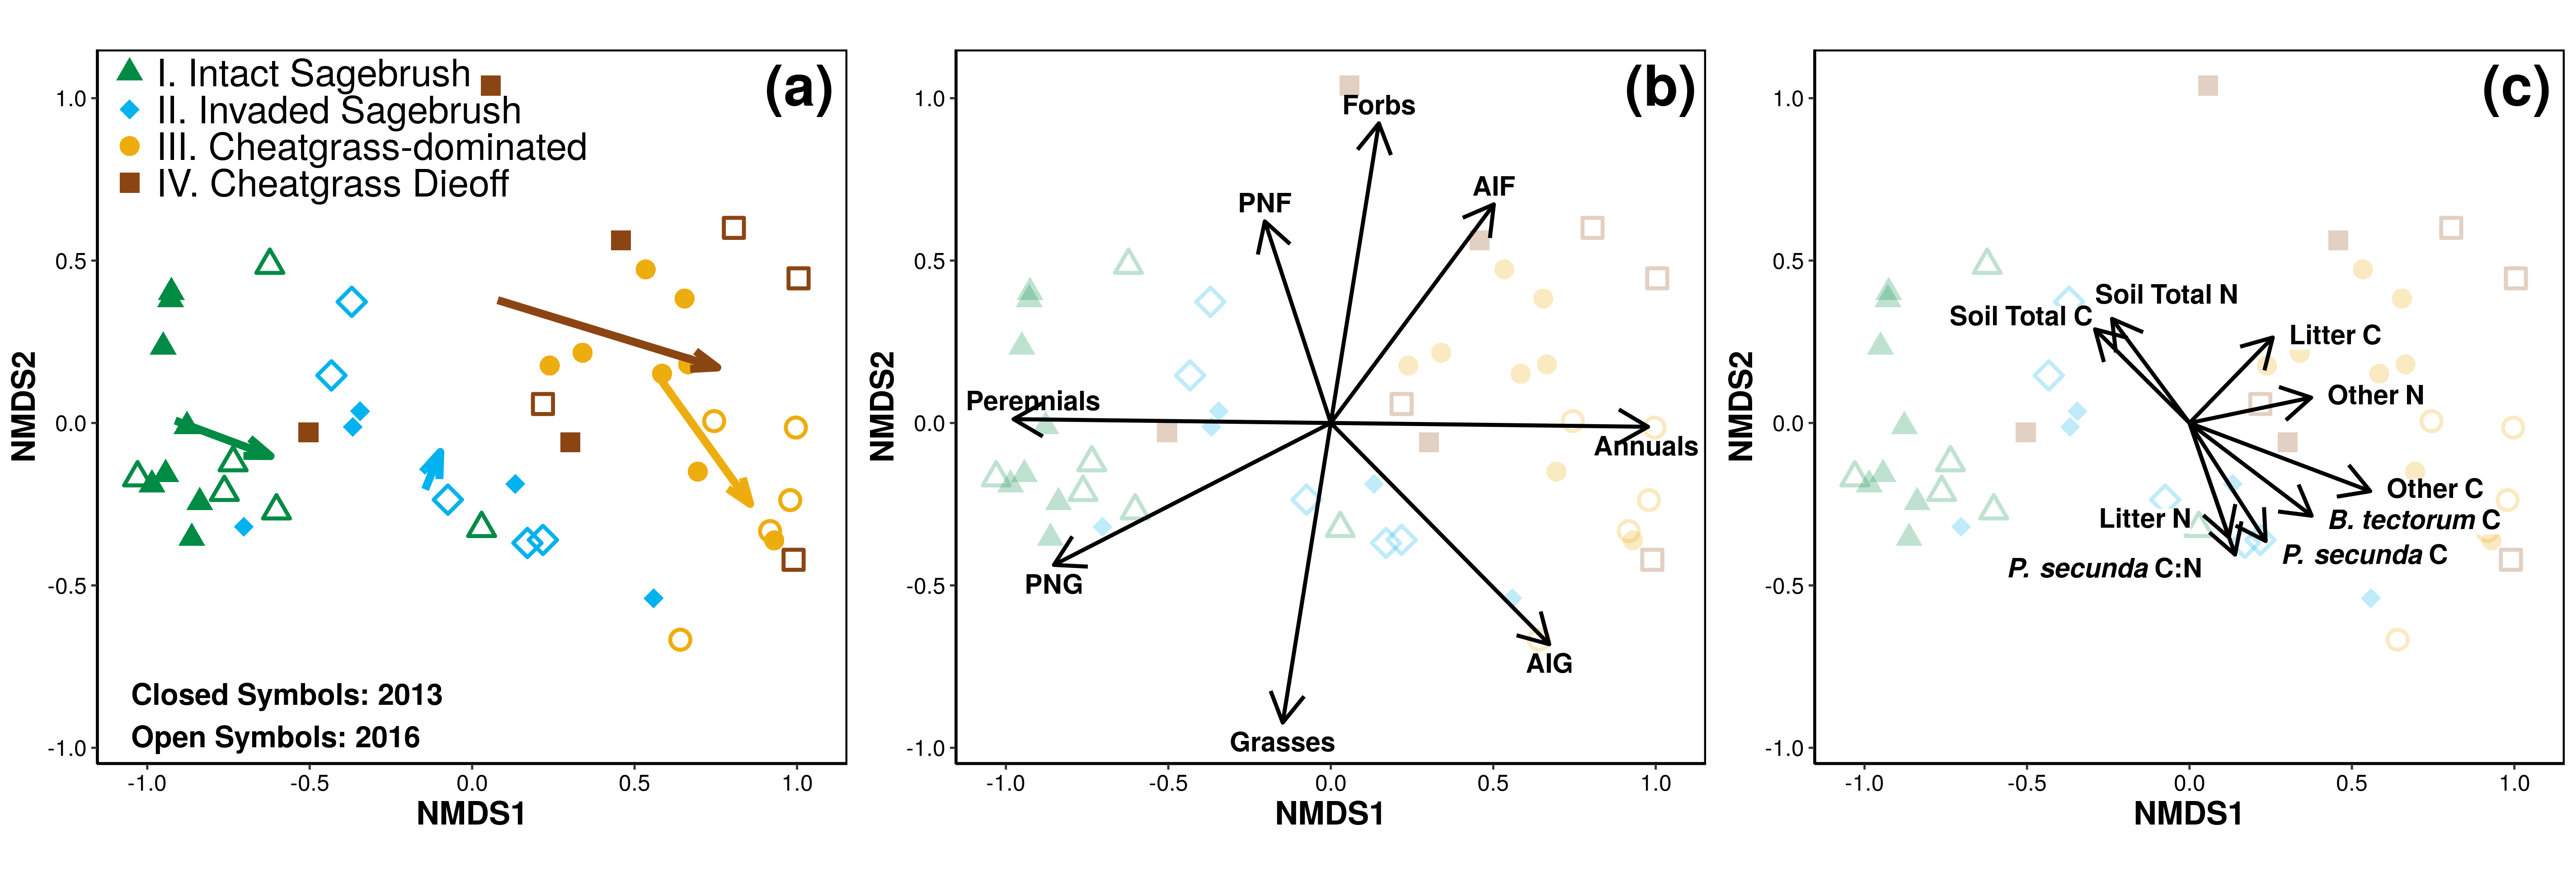
\includegraphics{figures/fig_2_nmds_3panel.png}
\caption{Non-metric multidimensional scaling ordination illustrating the differences in understory composition, and soil, plant and litter N and C between 2013 and 2016. Graphs illustrate (a), the mean change from 2013 to 2016 by invasion stage; (b), significant correlations (p \textless{} 0.05) of plant functional group cover with the ordination; and (c), significant correlations of soil, plant and litter nutrient concentrations with the ordination. The arrows in (a) represent the direction and magnitude of change. The length of each arrow in (b) and (c) corresponds to the R\(^2\) of the correlation. AIG = annual invasive grass cover; AIF = annual invasive forb cover; PNF = perennial native forb cover; PNG = perennial native grass cover.}
\end{figure}

\begin{table}

\caption{\label{tab:unnamed-chunk-3}Type III ANOVA results for soil total C and N, soil C:N ratio, soil nutrients, and litter and plant \%C, \%N, and C to N ratios. ANOVAs are based on mixed models with year and invasion stage as fixed effects, and site as the random effect. Denominator degrees of freedom (not shown) and F-statistics were calculated using the Kenward-Roger method}
\centering
\fontsize{8}{10}\selectfont
\begin{tabular}[t]{lrlrlrl}
\toprule
\multicolumn{1}{c}{ } & \multicolumn{2}{c}{Year} & \multicolumn{2}{c}{Invasion Stage} & \multicolumn{2}{c}{Year x Invasion Stage} \\
\cmidrule(l{3pt}r{3pt}){2-3} \cmidrule(l{3pt}r{3pt}){4-5} \cmidrule(l{3pt}r{3pt}){6-7}
 & F & P(>F) & F & P(>F) & F & P(>F)\\
\midrule
Soil Total N & 32.6 & <0.001 & 0.8 & 0.516 & 6.0 & 0.001\\
Soil Total C & 105.2 & <0.001 & 0.3 & 0.856 & 3.1 & 0.031\\
Soil C:N & 117.9 & <0.001 & 0.6 & 0.594 & 0.5 & 0.716\\
\addlinespace
Soil NO$_3$ & 765.7 & <0.001 & 1.5 & 0.256 & 4.5 & 0.005\\
Soil NH$_4$ & 104.0 & <0.001 & 1.9 & 0.172 & 2.3 & 0.085\\
Soil NH$_4$ + NO$_3$ & 363.6 & <0.001 & 1.8 & 0.182 & 2.3 & 0.085\\
\addlinespace
Litter N & 77.4 & <0.001 & 0.8 & 0.519 & 6.6 & <0.001\\
Litter C & 7.2 & 0.008 & 4.5 & 0.015 & 2.5 & 0.066\\
Litter C:N & 48.3 & <0.001 & 2.3 & 0.104 & 5.4 & 0.002\\
\addlinespace
\emph{Bromus} C & 128.9 & <0.001 & 7.4 & 0.002 & 4.9 & 0.003\\
\emph{Bromus} C:N & 173.8 & <0.001 & 0.7 & 0.563 & 2.1 & 0.101\\
\emph{Bromus} N & 163.8 & <0.001 & 1.4 & 0.264 & 3.3 & 0.023\\
\addlinespace
\emph{Poa} C & 3.1 & 0.081 & 0.6 & 0.628 & 0.4 & 0.726\\
\emph{Poa} C:N & 122.0 & <0.001 & 1.6 & 0.241 & 1.7 & 0.177\\
\emph{Poa} N & 248.3 & <0.001 & 3.7 & 0.037 & 11.8 & <0.001\\
\addlinespace
Other C & 20.8 & <0.001 & 5.6 & 0.006 & 4.5 & 0.005\\
Other C:N & 60.4 & <0.001 & 6.2 & 0.004 & 2.2 & 0.088\\
Other N & 59.2 & <0.001 & 5.9 & 0.004 & 3.0 & 0.035\\
\bottomrule
\end{tabular}
\end{table}

\hypertarget{soil-and-litter-characteristics}{%
\subsection{3.2 Soil and litter characteristics}\label{soil-and-litter-characteristics}}

Soil C, N, C:N ratios, and secondary soil nutrients were all lower in 2016 than in 2013 (Table 1). Few meaningful patterns existed among invasion stages for the soil variables (Table 1), but there were several variables with significant interactions between the years and invasion stages. In the intact sagebrush stage (I) total N content was similar in 2013 and 2016 but in the other stages total N content was higher in 2013 than 2016 (Figure 3a). A similar but weaker pattern occurred for soil total C (p=0.039; Figure 3b). Soil SO\(_4\) was lower for all invasion stages in 2016 except in stage IV, where it was similar for both years. (Figure 3d). Soil Ca was lower for all invasion stages in 2016 except in stage I, where it was similar for both years (Figure 3e). Litter N was higher in 2016 than in 2013 for stages I, II, and IV but did not differ in stage III (Figure 3g). Litter C and C:N were lower in 2016 than 2013 for stages I and II, but did not differ in stage III, while in stage IV C:N was lower in 2016 and C was similar in the two years (Tables 1, Figure 3h-i).

\begin{figure}
\centering
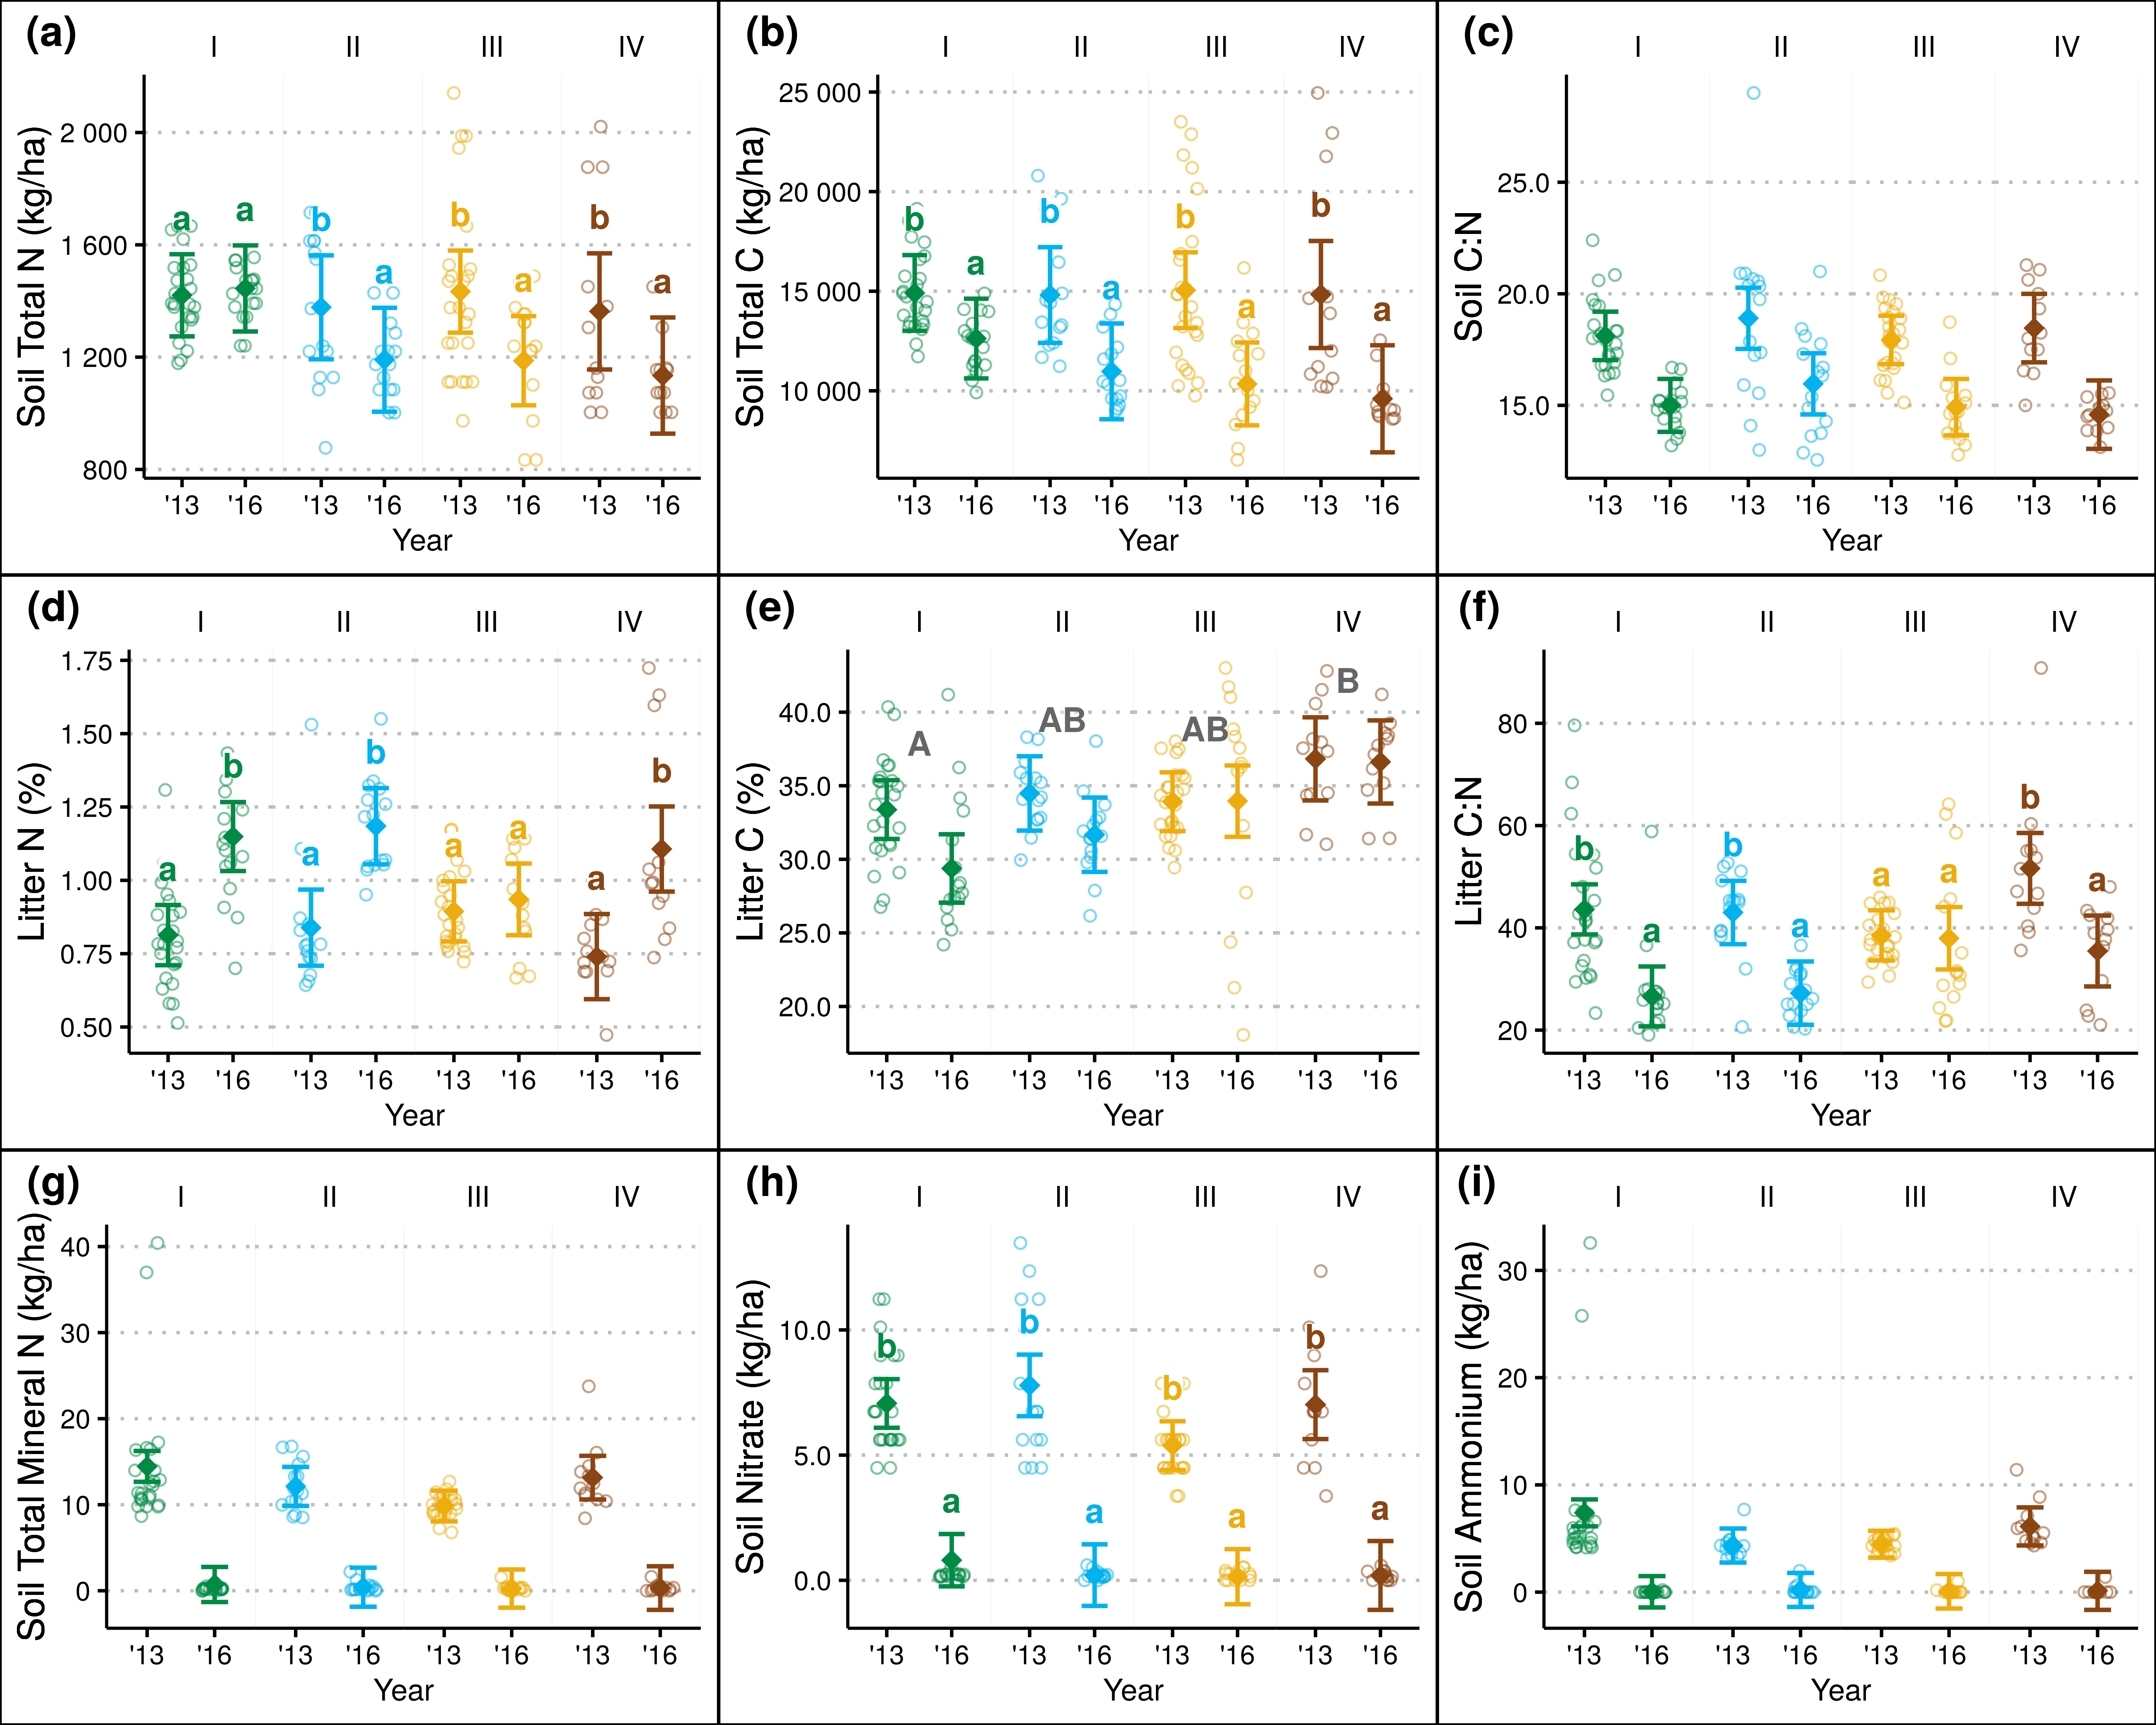
\includegraphics{figures/tidy_soilvars_year.png}
\caption{Effects of year and invasion stage on soil total C and N, soil C:N ratio (a-c), litter \%C, \%N, and C:N ratio (d-f), and soil total mineral N, nitrate, and ammonium (g-i). Open circles represent individual measurements. Diamonds and error bars represent the marginal means and 95\% confidence intervals estimated from the linear mixed models. Year was always significant. When the interaction between invasion stage and year is significant, colored lowercase letters above the bars illustrate differences between years within each invasion stage based on the Tukey Honest Significant Differences post-hoc test. Grey capital letters illustrate significant differences among invasion stages when the interaction was not significant.}
\end{figure}

Analyses of standard deviations of soil total C and N, litter \%C, \%N, and C:N ratios showed differences among invasion stage and year. When sites were grouped into the four invasion stages, within-site standard deviations differed only between stages I and IV for soil total C (Table S4). However, when sites were grouped by amount of \emph{A. tridentata} cover (stages I and II versus III and IV), within-site standard deviations in soil total C and soil C:N ratio were lower for stages III and IV than for stages I and II (Table 2). When the data were grouped by year, standard deviations of soil total N were higher in 2013, the dry year, while variation in litter N was higher in 2016, the wet year (Table 2).

\begin{table}

\caption{\label{tab:unnamed-chunk-4}Comparisons of stages I-II and stages III-IV and of the wet (2016) and dry (2013) years based on standard deviations calculated from three replicate samples from each site, averaged within each category. Letters indicate significant differences between grouped stages and years based on Kruskal-Wallis tests.}
\centering
\fontsize{8}{10}\selectfont
\begin{tabular}[t]{l>{\raggedleft\arraybackslash}p{1cm}>{\raggedright\arraybackslash}p{0.5cm}>{\raggedleft\arraybackslash}p{1cm}>{\raggedright\arraybackslash}p{0.5cm}|>{\raggedleft\arraybackslash}p{1cm}>{\raggedright\arraybackslash}p{0.5cm}>{\raggedleft\arraybackslash}p{1cm}>{\raggedright\arraybackslash}p{0.5cm}}
\toprule
 & Stages I-II &  & Stages III-IV &  & 2016 (Wet) &  & 2013 (Dry) & \\
\midrule
Soil Total N (kg/ha) & 96.2 &  & 85.4 &  & 59.7 & b & 116.3 & a\\
Soil Total C (kg/ha) & 1275.2 & a & 847.3 & b & 939.8 &  & 1184.1 & \\
Soil C:N & 1.3 & a & 0.7 & b & 0.9 &  & 1.2 & \\
\addlinespace
Litter N (\%) & 0.1 &  & 0.1 &  & 0.1 & a & 0.1 & b\\
Litter C (\%) & 2.8 &  & 2.5 &  & 3.2 &  & 2.2 & \\
Litter C:N & 5.9 &  & 6.6 &  & 6.7 &  & 5.9 & \\
\bottomrule
\end{tabular}
\end{table}

\hypertarget{plant-tissue-characteristics}{%
\subsection{3.3 Plant tissue characteristics}\label{plant-tissue-characteristics}}

Carbon concentrations of \emph{P. secunda} , \emph{B. tectorum} and other plants were higher in the wet year (2016) than the dry year (2013), and nitrogen concentrations were lower in the wet year. Because N concentrations were lower in the wet year, C:N ratios were higher (Figure 4, Table 1). \emph{B. tectorum} had lower C concentrations in stage I than all other stages in the dry year (2013) (Figure 4). \emph{P. secunda} had higher N concentrations in stage III than II in 2013, but N concentrations did not vary by invasion stage in 2016. Both species had higher C concentration in stage III than stages I and II and higher N concentrations in stage IV than in stages I and II. As a result, C:N ratios were lower in stage IV than in stages I and II. The contrast in nutrient concentrations for other plants between the shrub-dominated versus herbaceous-dominated invasion stages is likely due to the difference in species composition. The other plant species present in stages I and II were generally annual and perennial native forbs, while those in stages III and IV were mostly annual invasive forbs (Table S5).

\begin{figure}
\centering
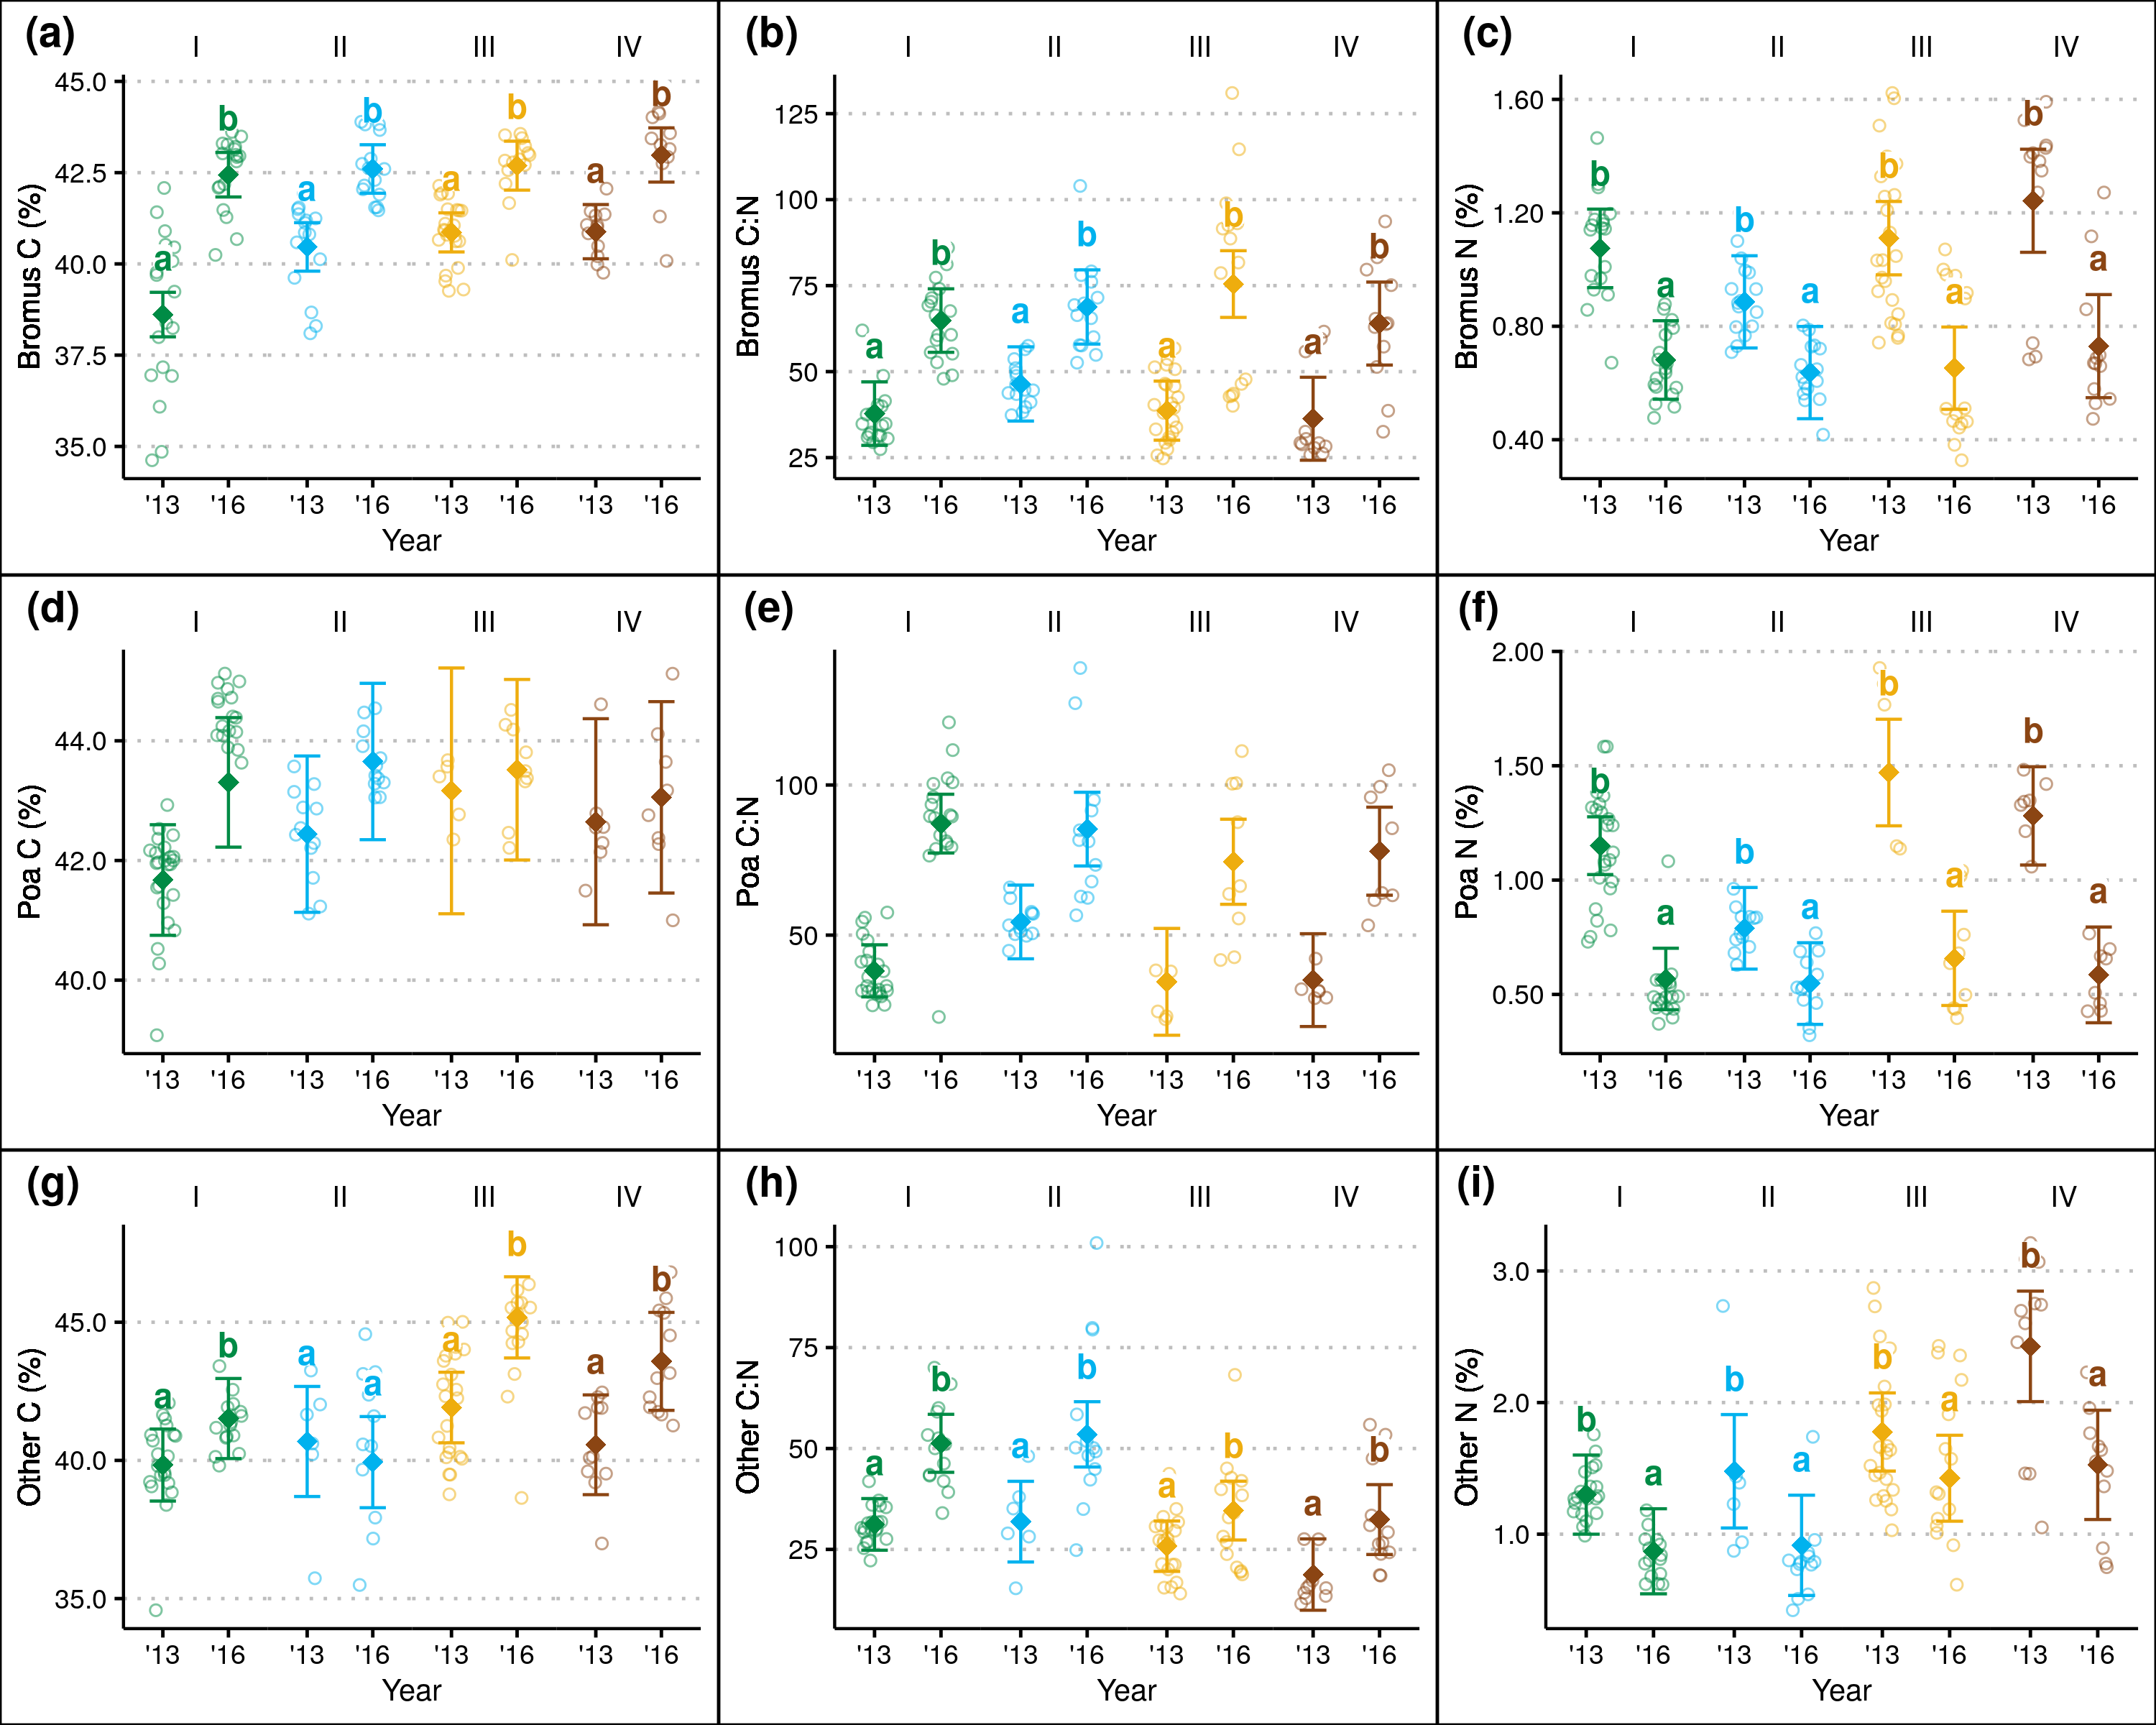
\includegraphics{figures/tidy_plantvars_year.png}
\caption{Effects of year and invasion stage on plant tissue C and N concentrations. Open circles represent individual measurements. Diamonds and error bars represent the marginal means and 95\% confidence intervals estimated from the linear mixed models. Year was always significant. When the interaction between invasion stage and year is significant, colored lowercase letters above the bars illustrate differences between years within each invasion stage based on the Tukey Honest Significant Differences post-hoc test. Grey capital letters illustrate significant differences among invasion stages when the interaction was not significant.}
\end{figure}

\hypertarget{path-models-for-soil-total-nitrogen-and-carbon}{%
\subsection{3.4 Path models for soil total nitrogen and carbon}\label{path-models-for-soil-total-nitrogen-and-carbon}}

Path models fit well with values approaching 1 for measures of fit (CFI, TLI) and values approaching 0 for measures of error (RMSEA, SRMR, Table S6). Covariance matrices for each path model are in the supplemental material in Tables S7-S8. The models for soil total C and N were quite different when split between the shrub-dominated invasion stages (I \& II) and those dominated by invasive annuals (III \& IV). The model for stages I \& II had many direct climate effects on soil total C and N, with indirect effects through the litter C:N ratio and perennial native grass cover. In contrast, in the model for the later invasion stages soil total C and N were strongly influenced by annual invasive grass cover.

\begin{figure}
\centering
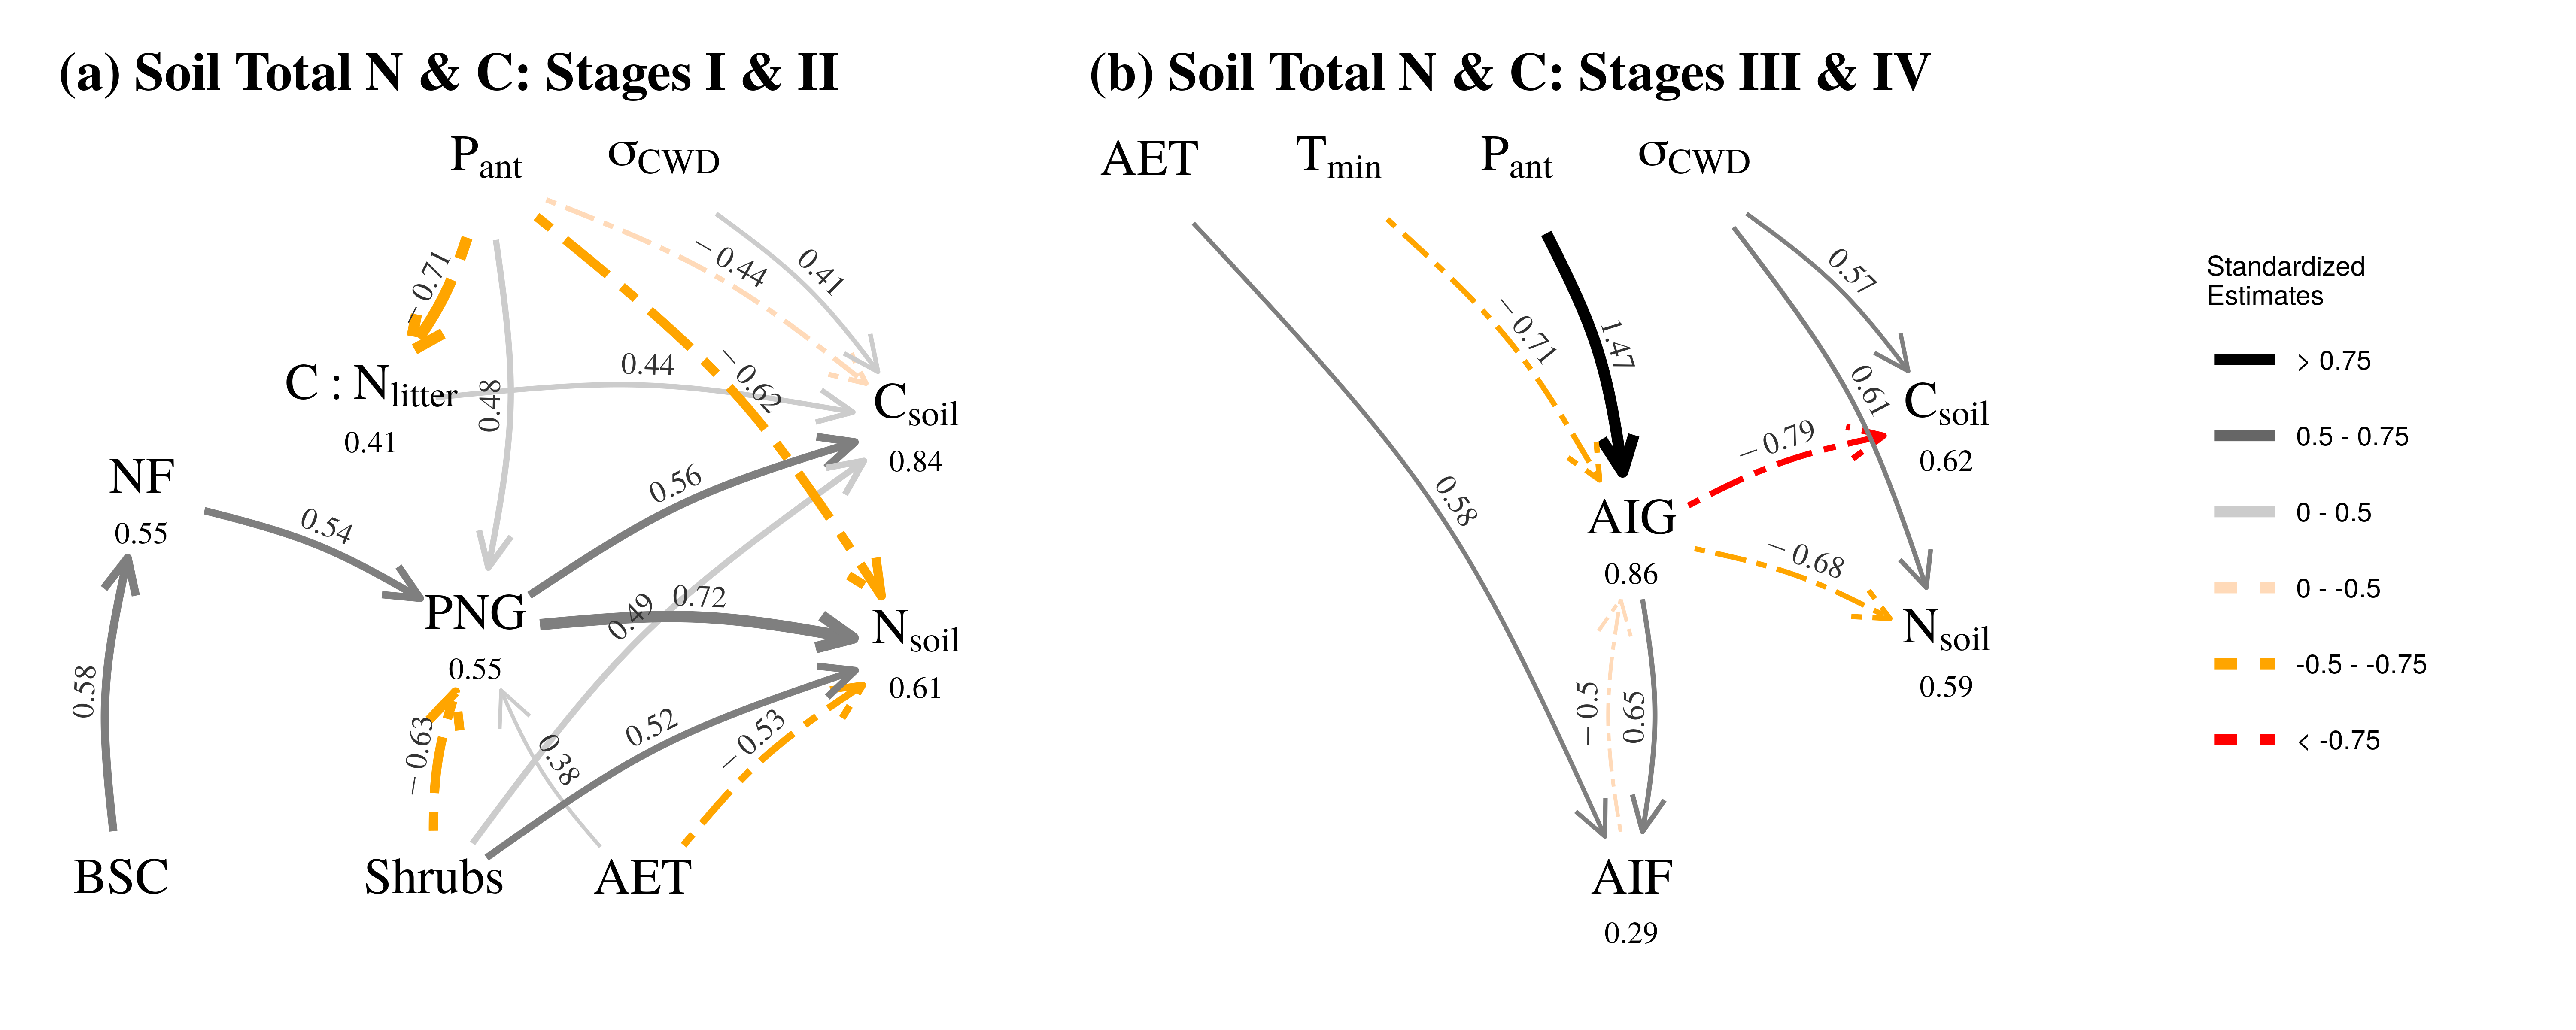
\includegraphics{figures/newsems/soilcn_panel.png}
\caption{Path models predicting soil total carbon and nitrogen for (a) invasion stages I \& II, and (b) invasion stages III \& IV. Paths are based on bootstrapped standardized solutions (R=5000); those with bootstrapped confidence intervals crossing zero have been omitted. The numbers along each path are the median standardized coefficients, which also correspond to the line widths. The numbers below each endogenous or response variable are the median bootstrapped R\(^2\) values. Gray and black lines indicate positive relationships; orange and red lines indicate negative relationships. AET = actual evapotranspiration; T\(_\text{min}\) = minimum temperature; P\(_\text{ant}\) = antecedent precipitation; \(\sigma_\text{CWD}\) = standard deviation of climatic water deficit; AIF = annual invasive forb cover; Litter = litter cover; NF = native forb cover; AIG = annual invasive grass cover; PNG = perennial native grass cover; Shrubs = shrub cover; BSC = biological soil crust cover; N\(_\text{soil}\)= soil total nitrogen; C\(_\text{soil}\) = soil total carbon.}
\end{figure}

The model for invasion stages I and II explained 84\% of the variation for soil total C and 61\% for soil total N (Figure 5a). Litter C:N, PNG, shrub cover, and \(\sigma_\text{CWD}\) were positively related to soil total C. P\(_\text{ant}\) was negatively related to soil total C, but positively influenced PNG and negatively influenced litter C:N. The indirect and total effects of P\(_\text{ant}\) on soil total C mediated through litter C:N were negative, while the effects of P\(_\text{ant}\) mediated through PNG were neutral (Table 3). Shrub cover and PNG had positive effects on soil total N, while P\(_\text{ant}\) and AET had negative effects. The indirect effects of P\(_\text{ant}\) and AET mediated through PNG were both neutral.

The model for invasion stages III \& IV explained 62\% of the variation for soil total C and 59\% of the variation for soil total N (Figure 5b). Both soil total C and soil total N were positively influenced by \(\sigma_\text{CWD}\) and negatively influenced by AIG. The indirect and total effects of P\(_\text{ant}\) mediated through AIG were negative for total soil C and neutral for soil total N. The indirect effects of T\(_\text{min}\) mediated through AIG were positive for soil total C and neutral for soil total N (Table 4). The total effect of T\(_\text{min}\) mediated through AIG was positive.

\begin{table}

\caption{\label{tab:unnamed-chunk-5}Indirect and total effects of climatic variables on soil total nitrogen and carbon for stages III and IV. Values are the median of the bootstrapped (n=5000) coefficients, and stars indicate that the 95 percent confidence intervals did not cross zero. Median coefficients for the direct effects are displayed in Figure 5b.}
\centering
\fontsize{8}{10}\selectfont
\begin{tabular}[t]{llrlrll}
\toprule
 & Mediator(s) & Soil C &  & Soil N &  & Invasion Stages\\
\midrule
\addlinespace[0.3em]
\multicolumn{7}{l}{\textbf{Actual Evapotranspiration}}\\
\hspace{1em}Indirect (single pathway) & PNG & 0.19 &  & 0.25 &  & I and II\\
\hspace{1em}Total & PNG & -0.06 &  & -0.26 &  & I and II\\
\addlinespace[0.3em]
\multicolumn{7}{l}{\textbf{Antecedent Precipitation}}\\
\hspace{1em}Indirect (single pathway) & LCN & -0.30 & * &  &  & I and II\\
\hspace{1em}Indirect (single pathway) & PNG & 0.26 &  & 0.34 &  & I and II\\
\hspace{1em}Total & LCN & -0.74 & * &  &  & I and II\\
\hspace{1em}Total & PNG & -0.17 &  & -0.27 &  & I and II\\
\midrule
\addlinespace[0.3em]
\multicolumn{7}{l}{\textbf{Actual Evapotranspiration}}\\
\hspace{1em}Indirect (multiple pathways) & AIF AIG & -0.10 &  & -0.08 &  & III and IV\\
\hspace{1em}Indirect (single pathway) & AIG & -0.31 &  & -0.27 &  & III and IV\\
\hspace{1em}Total & AIF AIG & -0.17 &  & -0.14 &  & III and IV\\
\hspace{1em}Total & AIG & 0.08 &  & 0.13 &  & III and IV\\
\addlinespace[0.3em]
\multicolumn{7}{l}{\textbf{Antecedent Precipitation}}\\
\hspace{1em}Indirect (single pathway) & AIG & -1.20 & * & -1.00 &  & III and IV\\
\hspace{1em}Total & AIG & -0.70 & * & -0.50 &  & III and IV\\
\addlinespace[0.3em]
\multicolumn{7}{l}{\textbf{Minimum Temperature}}\\
\hspace{1em}Indirect (single pathway) & AIG & 0.55 & * & 0.48 &  & III and IV\\
\hspace{1em}Total & AIG &  &  & 0.54 & * & III and IV\\
\bottomrule
\end{tabular}
\end{table}

\hypertarget{discussion}{%
\section{4. DISCUSSION}\label{discussion}}

Here we demonstrate that the well-documented sensitivity of herbaceous cover to inter-annual climatic variability (\protect\hyperlink{ref-Felton2021}{Felton et al., 2021}; \protect\hyperlink{ref-Hallett2019}{Hallett et al., 2019}; \protect\hyperlink{ref-Pilliod2017}{Pilliod et al., 2017}; \protect\hyperlink{ref-Witwicki2016}{Witwicki et al., 2016}) mediates the effects of progressive invasion of exotic annual grasses and changes in plant functional group composition on soil total C and N, and plant tissue C and N. Our NMS ordination indicated that differences in community composition were affecting soil total N and total C pools, while our linear mixed models indicated that year effects were a primary driver. Using path models to incorporate the effects of interannual climatic variability, we showed that different variables were determining soil total C and soil total N in the different invasion stages. Furthermore, climate-driven differences in herbaceous plant cover drove soil total C and soil total N in different directions depending on the composition of the herbaceous vegetation, with annual invaders resulting in losses of soil total C and soil total N, and native perennials resulting in increases (Figure 5).

To our knowledge, this is the first study in this system where multiple sites were sampled across a broad geographic extent, and both the stage of invasion and interannual climatic variability were taken into account. Prior studies on the relationship between \emph{B. tectorum} invasion and soil total N and C pools are conflicting, with reports of both higher (\protect\hyperlink{ref-Booth2003}{Booth et al., 2003}; \protect\hyperlink{ref-Gasch2013}{Gasch et al., 2013}; \protect\hyperlink{ref-Hooker2008biogeochem}{Hooker et al., 2008}) and lower (\protect\hyperlink{ref-Rau2011}{Rau et al., 2011}; \protect\hyperlink{ref-Stark2015}{Stark \& Norton, 2015}) levels after invasion. Failure to adequately account for spatial and interannual climate variability within an ecosystem is a common shortcoming in ecological research (\protect\hyperlink{ref-Werner2020}{Werner et al., 2020}) and helps explain the discrepancies in prior studies.

\hypertarget{annual-grass-invasion-and-loss-of-shrubs-reduce-and-homogenize-soil-total-n-and-c}{%
\subsection{4.1 Annual grass invasion and loss of shrubs reduce and homogenize soil total N and C}\label{annual-grass-invasion-and-loss-of-shrubs-reduce-and-homogenize-soil-total-n-and-c}}

The path model for invasion stages III and IV indicated direct positive relationships between climatic variables and AIG cover, and direct negative relationships between AIG cover and soil total N and soil total C (Figure 5b). It is likely that the observed interactions between invasion stage and year effects (Table 1) are the result of climate amplifying the negative effect of annual grass productivity on soil total N and soil total C in stages III and IV. Our finding that increased annual grass cover was associated with soil N and soil total C losses in invasion stages lII and IV in the wetter year is consistent with an emerging consensus that the rate of nutrient cycling is likely higher in \emph{B. tectorum}-invaded environments in the Great Basin, and this is amplified in higher moisture years. One mechanism for faster nutrient cycling under \emph{B. tectorum} in favorable years may be increased root exudation of N into the soil by \emph{B. tectorum} (\protect\hyperlink{ref-Morris2016}{Morris et al., 2016}), which initiates a self-reinforcing feedback that facilitates \emph{B. tectorum} growth (\protect\hyperlink{ref-Blank2016}{Blank et al., 2016}; \protect\hyperlink{ref-OConner2015}{O'Conner et al., 2015}). Increased nutrient cycling can lead to labile N and C removal from near surface soil layers via percolation, respiration, denitrification, and runoff (\protect\hyperlink{ref-Austin2004}{Austin et al., 2004}; \protect\hyperlink{ref-Norton2004}{J. B. Norton et al., 2004}). In drier years, water from smaller precipitation events that does not provide sufficient moisture for plants to activate is still used by soil microbes to mineralize N and C (\protect\hyperlink{ref-Dijkstra2012}{Dijkstra et al., 2012}; \protect\hyperlink{ref-Evans2013}{S. E. Evans \& Burke, 2013}; \protect\hyperlink{ref-Fierer2003}{Fierer et al., 2003}; \protect\hyperlink{ref-Fierer2002}{Fierer \& Schimel, 2002}).

The loss of biological soil crust (BSC) due to soil disturbance and fire often accompanies \emph{B. tectorum} invasion, and further reduces the capacity of invaded sites to retain soil N and C. At our study sites, BSC cover was lower at the invaded sagebrush stage (II) than in the uninvaded stage, and essentially absent at cheatgrass-dominated (III) and cheatgrass die-off (IV) stages (Table S5). In addition to providing N input (\protect\hyperlink{ref-Belnap2016}{Belnap et al., 2016}; \protect\hyperlink{ref-Condon2018}{Condon \& Pyke, 2018}; \protect\hyperlink{ref-Weber2016}{Weber et al., 2016}), BSC reduces the rate of soil drying, and thus gives plants more time to activate and uptake newly available resources (\protect\hyperlink{ref-Austin2004}{Austin et al., 2004}). The loss of BSC as a source of N input, combined with increased nutrient cycling leading to N and C exiting the system, may add up to significant yearly losses in near-surface soils (\protect\hyperlink{ref-Austin2004}{Austin et al., 2004}).

The lack of shrub cover and uniform distribution of annual herbaceous plants at our sites in invasion stages III and IV is common post-fire and leads to the loss of ``islands of fertility'' (\protect\hyperlink{ref-Austin2004}{Austin et al., 2004}; \protect\hyperlink{ref-Bechtold2007}{Bechtold \& Inouye, 2007}; \protect\hyperlink{ref-Doescher1984}{Doescher et al., 1984}; \protect\hyperlink{ref-Evans2001}{R. D. Evans et al., 2001}; \protect\hyperlink{ref-Germino2018}{Germino et al., 2018}). We found statistically lower within-site variability of soil total C and soil C:N ratios in invasion stages that had lost shrub cover (Table 2). Lower resource heterogeneity reduces the availability and diversity of niches that species can occupy, making it harder for native species to reestablish (\protect\hyperlink{ref-Melbourne2007}{Melbourne et al., 2007}; \protect\hyperlink{ref-Tilman2004}{Tilman, 2004}). Thus, a reduction in within-site variability and homogenization of soil total C, as we observed here, may contribute to the continued long-term dominance of invasive annual plants.

\hypertarget{soil-plant-and-litter-c-and-n-concentrations-are-strongly-influenced-by-interannual-climate-variability}{%
\subsection{4.2 Soil, plant and litter C and N concentrations are strongly influenced by interannual climate variability}\label{soil-plant-and-litter-c-and-n-concentrations-are-strongly-influenced-by-interannual-climate-variability}}

Interannual climate variability affected every variable we measured: soil total C, soil total N, and the C:N ratios of litter and soil, and the tissues of \emph{P. secunda} , \emph{B. tectorum}, and other plants (Table 1, Figures 3-6). The large interannual differences in soil total C (Figure 3b) were unexpected, because soil organic C is usually considered to be fairly stable (but see \protect\hyperlink{ref-Lehmann2015}{Lehmann \& Kleber, 2015}; \protect\hyperlink{ref-Morgan2016}{Morgan et al., 2016}). In sagebrush ecosystems, soil water content is the primary driver of soil C mineralization (\protect\hyperlink{ref-Norton2012}{Norton et al., 2012}). When soil is wet, C cycling rates can be an order of magnitude greater than when soil is dry (\protect\hyperlink{ref-Saetre2005}{Saetre \& Stark, 2005}). Increased litter inputs associated with \emph{B. tectorum} invasion are associated with higher labile C in the top 10 cm and higher C mineralization rates (\protect\hyperlink{ref-Norton2012}{Norton et al., 2012}). In addition to losses from higher rates of soil respiration, this increased nutrient cycling may be leading to significant C losses through vertical movement of labile C from the top 0-10 cm sampled here to deeper soil depths (\protect\hyperlink{ref-Nagy2021}{Nagy et al., 2021}).

The cover and tissue nutrient content of the herbaceous plants were strongly influenced by interannual climatic variability (Figure 4). The resulting effect on litter chemistry may have regional scale consequences for fire risk and nutrient cycling. Plant biomass produced in dry periods becomes litter with low C:N ratios (\protect\hyperlink{ref-Evans2013}{S. E. Evans \& Burke, 2013}), which may persist for 2-3 years (\protect\hyperlink{ref-Pilliod2017}{Pilliod et al., 2017}). This can lead to increased rates of nutrient cycling and, thus, loss of mineralized N through leaching and gaseous loss of CO\(_2\), nitrification of NH\(_4\), and denitrification of NO\(_3\) when soil moisture is available (\protect\hyperlink{ref-Austin2004}{Austin et al., 2004}; \protect\hyperlink{ref-Evans2013}{S. E. Evans \& Burke, 2013}). In contrast, biomass produced in wetter periods becomes litter with higher C:N ratios. In the wet period, litter C:N was higher, \emph{B. tectorum} and \emph{P. secunda} C:N ratios were universally higher, and other plant C:N ratios were higher in invasion stages III and IV. The layer of dead and cured fine fuel created by the pulse of growth in wet years will potentially persist longer than the fuel produced in dry years, because litter with higher C:N ratios may decompose more slowly (\protect\hyperlink{ref-Grootemaat2015}{Grootemaat et al., 2015}; \protect\hyperlink{ref-Pausas2017}{Pausas et al., 2017}). Consequently, in wet years there is not only an increase in fine fuel biomass, but those fine fuels may be more flammable and take longer to decompose.

\hypertarget{drivers-of-soil-c-and-n-differ-with-invasion-stage}{%
\subsection{4.3. Drivers of soil C and N differ with invasion stage}\label{drivers-of-soil-c-and-n-differ-with-invasion-stage}}

Changes in species composition and simplification of plant community structure to a single herbaceous cover layer results in different pathways through which C and N travel. In all stages, the strongest direct predictors of C and N were abundance of the dominant grass type, i.e., PNG in stages I and II, and AIG in stages III and IV (Figure 5). In stages I and II, PNG had positive relationships with soil total N and soil total C, and the negative effect of higher water availability on soil total N and C was dampened by its positive influence on PNG cover. In these stages, sites with higher cover of shrubs, BSC, NF, and PNG were all associated with higher soil total N and C. This agrees with prior work indicating that sagebrush communities sequester C (\protect\hyperlink{ref-Prater2006}{Prater et al., 2006}), but that their ability to sequester C declines as the cover of key ecosystem components declines. In stages III and IV, the simplified species composition yielded a simple path model centered around a single pathway through AIG. In these sites, P\(_\text{ant}\) led to higher AIG which led to lower soil total N and soil total C. In contrast to \emph{Artemisia}-dominated stages I and II, the negative effect of higher water availability on soil total N and soil total C was amplified by its effect on the abundance of AIG, agreeing with \protect\hyperlink{ref-Prater2006}{Prater et al.} (\protect\hyperlink{ref-Prater2006}{2006}) who found \emph{B. tectorum} monocultures to be a net C source.

Litter chemistry and abundance is known to change after invasion with important consequences for soil nutrient cycling \protect\hyperlink{ref-Norton2008}{Norton et al.} (\protect\hyperlink{ref-Norton2008}{2008}). Because the vast majority of litter is dead plant material from the previous growing season, litter C:N ratios are reflective of the conditions of the preceding growing season. Here, litter C:N ratios operated differently between the soil total C and soil total N path models. In stages I and II litter C:N ratio was positively related to soil total C. Antecedent precipitation drove decreases in both soil total C, and litter C:N ratios, and higher litter C:N ratios amplified the effect of P\(_\text{ant}\) on soil total C (Table 4). \protect\hyperlink{ref-Huber2019}{Huber et al.} (\protect\hyperlink{ref-Huber2019}{2019}) also found that increases in winter rainfall can turn soil under sagebrush plants into a net C source. In stages III and IV, litter C:N ratio was not a significant part of the model, perhaps because the litter layer was composed mainly \emph{B. tectorum} detritus, and the C:N ratio did not differ between years.

\hypertarget{implications-for-management}{%
\subsection{4.4 Implications for management}\label{implications-for-management}}

Our results indicate that reductions in aboveground carbon storage resulting from the loss of shrubs (\protect\hyperlink{ref-Fusco2019}{Fusco et al., 2019}) are accompanied by belowground carbon losses. These losses may increase over time with ongoing climate change and progressive conversion to annual grass dominance. In the Great Basin, temperature has increased by 1 degree Celsius above historic averages and is projected to increase by 2-6 degrees Celsius by 2100 (\protect\hyperlink{ref-Bradford2020}{Bradford et al., 2020}; \protect\hyperlink{ref-melillo2014}{Melillo et al., 2014}). Future projections of precipitation are mixed, but models agree that there will be higher interannual variability (\protect\hyperlink{ref-Bradford2020}{Bradford et al., 2020}). These trends are resulting in high climate suitability for \emph{B. tectorum} and other annual invaders (\protect\hyperlink{ref-Mcmahon2021}{McMahon et al., 2021}) as well as increased risk of large-scale wildfire across much of the area (\protect\hyperlink{ref-Brown2021}{Brown et al., 2021}; \protect\hyperlink{ref-Gao2021}{Gao et al., 2021}). Sagebrush shrublands are currently experiencing among the largest wildfires in the western U.S. (\protect\hyperlink{ref-Brooks2015}{Brooks et al., 2015}; \protect\hyperlink{ref-Dennison2014}{Dennison et al., 2014}), loss of the dominant shrub species (fire-intolerant \emph{A. tridentata}), and active conversion to grasslands dominated by invasive annuals. This conversion will likely result in progressive decreases in carbon storage if our ability to restore these ecosystems does not improve (\protect\hyperlink{ref-Arkle2014}{Arkle et al., 2014}; \protect\hyperlink{ref-Knutson2014}{Knutson et al., 2014}).

Restoring sagebrush ecosystems and maintaining their capacity to store and retain carbon and soil nutrients is becoming more challenging as temperatures and interannual climate variability increase. After wildfire in many sagebrush ecosystems, there is a short temporal window outside of which restoration is not likely to succeed. In the first 1-3 years after fire, \emph{B. tectorum} typically has relatively low density and cover and competition with seeded species is low (\protect\hyperlink{ref-Chambers2014rem}{Chambers et al., 2014}; \protect\hyperlink{ref-Urza2017}{Urza et al., 2017}, \protect\hyperlink{ref-Urza2019}{2019}). The soil resource islands beneath shrubs increase post-fire establishment of seeded perennials {[}\protect\hyperlink{ref-Germino2018}{Germino et al.} (\protect\hyperlink{ref-Germino2018}{2018})\} and can persist for several years after fire (\protect\hyperlink{ref-Bechtold2007}{Bechtold \& Inouye, 2007}). Our results indicate that after conversion to annual grass dominance, these resource islands eventually disappear. The homogenization and depletion of soil nutrient pools may negatively affect establishment processes by reducing both resource availability (\protect\hyperlink{ref-Davis2000}{Davis et al., 2000}) and niche diversity (\protect\hyperlink{ref-Fukami2015}{Fukami, 2015}; \protect\hyperlink{ref-Melbourne2007}{Melbourne et al., 2007}). Strategies for overcoming the post-fire establishment bottleneck include optimizing the timing of restoration by anticipating cooler and wetter years and taking advantage of them when they occur (\protect\hyperlink{ref-Bradford2018}{Bradford et al., 2018}; \protect\hyperlink{ref-Hardegree2018}{Hardegree et al., 2018}; \protect\hyperlink{ref-Shriver2018}{Shriver et al., 2018}). Restoration techniques for addressing interannual climate variability include seed priming and coating to shorten germination times and maximize water availability for seedling establishment (\protect\hyperlink{ref-Pedrini2020}{Pedrini et al., 2020}). Various site preparation techniques also increase seedling establishment (\protect\hyperlink{ref-Farrell2021}{Farrell et al., 2021}; \protect\hyperlink{ref-Herriman2016}{Herriman et al., 2016}), and methods used in more arid systems for increasing soil water availability, such as soil imprinting (\protect\hyperlink{ref-Doherty2020}{Doherty et al., 2020}), may be beneficial.

Selecting restoration species that are adapted not only to increased temperatures and aridity but also interannual climate variability around these trends may increase restoration success (\protect\hyperlink{ref-bradley_st_clair_genetic_2013}{Bradley St. Clair et al., 2013}; \protect\hyperlink{ref-Gibson2016eva}{A. L. Gibson et al., 2016}). Current approaches use climate-informed seed transfer zones to minimize the possibility of introducing maladapted genotypes (\protect\hyperlink{ref-Bower2014}{Bower et al., 2014}; \protect\hyperlink{ref-Gibson2019}{A. Gibson et al., 2019}). It may be necessary to modify these approaches to use current climate to determine suitability but use future climate scenarios to help determine the species and zone of application (\protect\hyperlink{ref-Richardson2018}{Richardson \& Chaney, 2018}; \protect\hyperlink{ref-Shryock2018}{Shryock et al., 2018}).

In many areas sagebrush restoration, regardless of the technique, is unlikely to succeed because of prolonged annual grass dominance or temperature increases that have already occurred (\protect\hyperlink{ref-Germino2018}{Germino et al., 2018}; \protect\hyperlink{ref-Shriver2018}{Shriver et al., 2018}, \protect\hyperlink{ref-Shriver2019}{2019}). Our results indicate that after invasive annuals have displaced perennials the system is more sensitive to interannual climate variability and more susceptible to soil C and N losses. Thus, it may be prudent for land management in these areas to shift the focus from restoring particular species to restoring plant community structure -- deep-rooted shrubs, grasses, and forbs (\protect\hyperlink{ref-Balazs2020}{Balazs et al., 2020}; \protect\hyperlink{ref-bradley_st_clair_genetic_2013}{Bradley St. Clair et al., 2013}; \protect\hyperlink{ref-Laughlin2014}{Laughlin, 2014}). Restoration with native species other than sagebrush may not have the same habitat benefits as successful sagebrush restoration. However, if native species can be established that compete effectively with invasive annuals, tolerate fire, and persist in future climate conditions (\protect\hyperlink{ref-Butterfield2017}{Butterfield et al., 2017}), the system may be able to maintain C sequestration, soil fertility, and soil heterogeneity in the face of interannual climate variability.

\hypertarget{implications-for-future-research}{%
\subsection{4.5 Implications for future research}\label{implications-for-future-research}}

Future research should investigate the effects of annual grass invasion on ecosystem function in different stages of invasion at larger spatial extents and with enough repeated measurements to capture long-term trends in the context of interannual variability (\protect\hyperlink{ref-Cusser2021}{Cusser et al., 2021}). Functional components include stocks of above- and belowground biomass, soil total C and N storage and soil water storage. Annual or subannual data collected at temporal extents long enough to capture the full range of variability are necessary to disentangle long-term trends of these functional components from the confounding effects of interannual variability (\protect\hyperlink{ref-Werner2020}{Werner et al., 2020}), time since invasion, time since disturbance and soil characteristics (\protect\hyperlink{ref-Austin2004}{Austin et al., 2004}; \protect\hyperlink{ref-Noy-Meir1973}{Noy-Meir, 1973}). Some prior studies had well defined invasion stages (\protect\hyperlink{ref-Rau2011}{Rau et al., 2011}), or a well-defined time of introduction (\protect\hyperlink{ref-Stark2015}{Stark \& Norton, 2015}), but to our knowledge no study has adequately captured the range of interannual variability in this system. Time since initial introduction may not always be feasible to ascertain, but annual grass invasions initiated during the satellite record may be detected from seasonal differences in NDVI (\protect\hyperlink{ref-Boyte2019}{Boyte et al., 2019}; \protect\hyperlink{ref-Bradley2006}{Bradley \& Mustard, 2006}). Time since the loss of woody plant cover may be determined from satellite-derived datasets of fire occurrence (\protect\hyperlink{ref-Balch2020fired}{Balch et al., 2020}; \protect\hyperlink{ref-Hawbaker2017}{Hawbaker et al., 2017}) and functional group fractional cover (\protect\hyperlink{ref-Jones2018}{Jones et al., 2018}). Understanding the inter- and intra-annual variability in each component of above- and belowground C and N pools and fluxes over decadal temporal extents will allow for the determination of rates of change at each site, rather than relying on space for time substitutions.

\hypertarget{conclusions}{%
\section{5. CONCLUSIONS}\label{conclusions}}

Episodic differences in temperature and water availability have predictable effects on \emph{B. tectorum} invasion and soil nutrients, but have seldom been adequately analyzed. Our results indicate that annual grass invasion changes mechanisms and pathways of nutrient cycling and carbon storage, especially after the loss of shrubs. While soil water content is perhaps the single most important factor in nutrient cycling in dryland ecosystems, our research illuminates some nuance. We found that the strength and direction of the effects of water availability on soil total C and N are dependent on plant functional group composition, because long-lived, deep-rooted plants tend to store nutrients belowground, while short-lived, shallow-rooted plants tend to extract nutrients. Thus, while changes in the mean and variation of water availability was the primary control, the effects of water availability on soil C and N were amplified by invasive annuals and dampened by native perennials. These changes in mechanisms and pathways of nutrient cycling and carbon storage that result from conversion from perennial to annual dominance will likely lead to the long-term depletion of soil resources and a decline in resource heterogeneity.

\hypertarget{acknowledgements}{%
\section{6. ACKNOWLEDGEMENTS}\label{acknowledgements}}

We are grateful to C. Nick Whittemore and Margaret Ryback for their tireless work in the field, and to Katlhleen Wiemer for helping in the lab. We thank R. Chelsea Nagy, Paul S. Verberg, Tim Seastedt, Caitlin T. White and two anonymous reviewers for helpful feedback that greatly improved the manuscript. We are also grateful to Dale Johnson, emeritus Professor, who helped design the study, and Mike Zeilinski, retired soil scientist, and the Winnemucca Bureau of Land Management field office for help selecting sampling locations. This project received funding from the Adam Kolff Memorial Research Fellowship Award and the University of Colorado's Undergraduate Research Opportunities Program, and was partly supported by the USDA Forest Service, Rocky Mountain Research Station. The authors declare no conflicts of interest.

\hypertarget{references}{%
\section{7. REFERENCES}\label{references}}

\hypertarget{refs}{}
\begin{CSLReferences}{1}{0}
\leavevmode\hypertarget{ref-Abatzoglou2013}{}%
Abatzoglou, J. T. (2013). {Development of gridded surface meteorological data for ecological applications and modelling}. \emph{International Journal of Climatology}, \emph{33}(1), 121--131. \url{https://doi.org/10.1002/joc.3413}

\leavevmode\hypertarget{ref-Allison2005}{}%
Allison, S. D., \& Vitousek, P. M. (2005). {Responses of extracellular enzymes to simple and complex nutrient inputs}. \emph{Soil Biology and Biochemistry}, \emph{37}(5), 937--944. \url{https://doi.org/10.1016/j.soilbio.2004.09.014}

\leavevmode\hypertarget{ref-Arkle2014}{}%
Arkle, R. S., Pilliod, D. S., Hanser, S. E., Brooks, M. L., Chambers, J. C., Grace, J. B., Knutson, K. C., Pyke, D. A., Welty, J. L., \& Wirth, T. A. (2014). Quantifying restoration effectiveness using multi-scale habitat models: {Implications} for sage-grouse in the {Great} {Basin}. \emph{Ecosphere}, \emph{5}(3), 1--32. \url{https://doi.org/10.1890/ES13-00278.1}

\leavevmode\hypertarget{ref-Austin2004}{}%
Austin, A. T., Yahdjian, L., Stark, J. M., Belnap, J., Porporato, A., Norton, U., Ravetta, D. A., \& Schaeffer, S. M. (2004). {Water pulses and biogeochemical cycles in arid and semiarid ecosystems}. \emph{Oecologia}, \emph{141}(2), 221--235. \url{https://doi.org/10.1007/s00442-004-1519-1}

\leavevmode\hypertarget{ref-Balazs2020}{}%
Balazs, K. R., Kramer, A. T., Munson, S. M., Talkington, N., Still, S., \& Butterfield, B. J. (2020). The right trait in the right place at the right time: {Matching} traits to environment improves restoration outcomes. \emph{Ecological Applications}, \emph{30}(4), e02110. https://doi.org/\url{https://doi.org/10.1002/eap.2110}

\leavevmode\hypertarget{ref-Balch2020fired}{}%
Balch, J. K., St. Denis, L. A., Mahood, A. L., MietKiewicz, N. P., Williams, T. M., McGlinchy, J., \& Cook, M. C. (2020). {FIRED (Fire Events Delineation): An open, flexible algorithm \& database of US fire events derived from the MODIS burned area product (2001-19)}. \emph{Remote Sensing}, \emph{12}, 3498. \url{https://doi.org/10.3390/rs12213498}

\leavevmode\hypertarget{ref-Bansal2016}{}%
Bansal, S., \& Sheley, R. L. (2016). {Annual grass invasion in sagebrush steppe: the relative importance of climate, soil properties and biotic interactions}. \emph{Oecologia}, \emph{181}(2), 543--557. \url{https://doi.org/10.1007/s00442-016-3583-8}

\leavevmode\hypertarget{ref-Bates2015}{}%
Bates, D., Mächler, M., Bolker, B., \& Walker, S. (2015). Fitting linear mixed-effects models using {lme4}. \emph{Journal of Statistical Software}, \emph{67}(1), 1--48. \url{https://doi.org/10.18637/jss.v067.i01}

\leavevmode\hypertarget{ref-Baughman2013}{}%
Baughman, O. W., \& Meyer, S. E. (2013). {Is \emph{Pyrenophora semeniperda} the cause of downy brome (\emph{Bromus tectorum}) die-offs?} \emph{Invasive Plant Science and Management}, \emph{6}(1), 105--111. \url{https://doi.org/10.1614/IPSM-D-12-00043.1}

\leavevmode\hypertarget{ref-Bechtold2007}{}%
Bechtold, H. A., \& Inouye, R. S. (2007). {Distribution of carbon and nitrogen in sagebrush steppe after six years of nitrogen addition and shrub removal}. \emph{Journal of Arid Environments}, \emph{71}(1), 122--132. \url{https://doi.org/10.1016/j.jaridenv.2007.02.004}

\leavevmode\hypertarget{ref-Belnap2016}{}%
Belnap, J., Stark, J. M., Rau, B. M., Allen, E. B., \& Phillips, S. (2016). {Soil moisture and biogeochemical factors Influence the distribution of annual \emph{Bromus} species}. In M. J. G. et al. (eds.) (Ed.), \emph{Exotic brome-grasses in arid and semiarid ecosystems of the western US} (pp. 227--256). \url{https://doi.org/10.1007/978-3-319-24930-8}

\leavevmode\hypertarget{ref-Blank2008}{}%
Blank, R. R. (2008). {Biogeochemistry of plant invasion: a case study with downy brome (\emph{Bromus tectorum})}. \emph{Invasive Plant Science and Management}, \emph{1}(2), 226--238. \url{https://doi.org/10.1614/IPSM-07-026.1}

\leavevmode\hypertarget{ref-Blank2016}{}%
Blank, R. R., Mackey, B., \& Morgan, T. (2016). {Do a native and two exotic grasses respond differently in soils conditioned by native vegetation versus an exotic grass?} \emph{Rhizosphere}, \emph{2}, 38--47. \url{https://doi.org/10.1016/j.rhisph.2016.08.004}

\leavevmode\hypertarget{ref-Booth2003}{}%
Booth, M. S., Stark, J. M., \& Caldwell, M. M. (2003). {Inorganic N turnover and availability in annual- and perennial-dominated soils in a Northern Utah shrub-steppe}. \emph{Biogeochemistry}, \emph{66}(3), 311--330.

\leavevmode\hypertarget{ref-Bower2014}{}%
Bower, A. D., Clair, J. B. St., \& Erickson, V. (2014). Generalized provisional seed zones for native plants. \emph{Ecological Applications}, \emph{24}(5), 913--919. \url{https://doi.org/10.1890/13-0285.1}

\leavevmode\hypertarget{ref-Boyte2019}{}%
Boyte, S. P., Wylie, B. K., \& Major, D. J. (2019). {Validating a time series of annual grass percent cover in the sagebrush ecosystem}. \emph{Rangeland Ecology and Management}, \emph{72}(2), 347--359. \url{https://doi.org/10.1016/j.rama.2018.09.004}

\leavevmode\hypertarget{ref-Bradford2018}{}%
Bradford, J. B., Betancourt, J. L., Butterfield, B. J., Munson, S. M., \& Wood, T. E. (2018). {Anticipatory natural resource science and management for a changing future}. \emph{Frontiers in Ecology and the Environment}, \emph{16}(5), 295--303. \url{https://doi.org/10.1002/fee.1806}

\leavevmode\hypertarget{ref-Bradford2018}{}%
Bradford, J. B., Betancourt, J. L., Butterfield, B. J., Munson, S. M., \& Wood, T. E. (2018). {Anticipatory natural resource science and management for a changing future}. \emph{Frontiers in Ecology and the Environment}, \emph{16}(5), 295--303. \url{https://doi.org/10.1002/fee.1806}

\leavevmode\hypertarget{ref-Bradford2014}{}%
Bradford, J. B., Schlaepfer, D. R., Lauenroth, W. K., \& Burke, I. C. (2014). {Shifts in plant functional types have time-dependent and regionally variable impacts on dryland ecosystem water balance}. \emph{Journal of Ecology}, \emph{102}(6), 1408--1418. \url{https://doi.org/10.1111/1365-2745.12289}

\leavevmode\hypertarget{ref-Bradford2020}{}%
Bradford, J. B., Schlaepfer, D. R., Lauenroth, W. K., \& Palmquist, K. A. (2020). Robust ecological drought projections for drylands in the 21st century. \emph{Global Change Biology}, \emph{26}(7), 3906--3919. \url{https://doi.org/10.1111/gcb.15075}

\leavevmode\hypertarget{ref-Bradley2018}{}%
Bradley, B. A., Curtis, C. A., Fusco, E. J., Abatzoglou, J. T., Balch, J. K., Dadashi, S., \& Tuanmu, M. N. (2018). {Cheatgrass (\emph{Bromus tectorum}) distribution in the intermountain Western United States and its relationship to fire frequency, seasonality, and ignitions}. \emph{Biological Invasions}, \emph{20}(6), 1493--1506. \url{https://doi.org/10.1007/s10530-017-1641-8}

\leavevmode\hypertarget{ref-Bradley2006}{}%
Bradley, B. A., \& Mustard, J. F. (2006). {Characterizing the landscape dynamics of an invasive plant and risk of invasion using remote sensing}. \emph{Ecological Applications}, \emph{16}(3), 1132--1147. \url{https://doi.org/10.1890/1051-0761(2006)016\%5B1132:CTLDOA\%5D2.0.CO;2}

\leavevmode\hypertarget{ref-bradley_st_clair_genetic_2013}{}%
Bradley St. Clair, J., Kilkenny, F. F., Johnson, R. C., Shaw, N. L., \& Weaver, G. (2013). Genetic variation in adaptive traits and seed transfer zones for \emph{pseudoroegneria spicata} (bluebunch wheatgrass) in the northwestern united states. \emph{Evolutionary Applications}, \emph{6}(6), 933--948. \url{https://doi.org/10.1111/eva.12077}

\leavevmode\hypertarget{ref-Brooks2015}{}%
Brooks, M. L., Matchett, J. R., Shinneman, D. J., \& Coates, P. S. (2015). \emph{Fire patterns in the range of the greater sage-grouse, 1984-2013 - {Implications} for conservation and management} (Report No. 2015-1167). \url{https://doi.org/10.3133/ofr20151167}

\leavevmode\hypertarget{ref-Brown2021}{}%
Brown, E. K., Wang, J., \& Feng, Y. (2021). {US} wildfire potential: A historical view and future projection using high-resolution climate data. \emph{Environmental Research Letters}, \emph{16}(3), 034060. \url{https://doi.org/10.1088/1748-9326/aba868}

\leavevmode\hypertarget{ref-Buckley2016}{}%
Buckley, Y. M., \& Catford, J. (2016). {Does the biogeographic origin of species matter? Ecological effects of native and non-native species and the use of origin to guide management}. \emph{Journal of Ecology}, \emph{104}, 4--17. \url{https://doi.org/10.1111/1365-2745.12501}

\leavevmode\hypertarget{ref-Butterfield2017}{}%
Butterfield, B. J., Copeland, S. M., Munson, S. M., Roybal, C. M., \& Wood, T. E. (2017). Prestoration: Using species in restoration that will persist now and into the future: {Prestoring} for climate change. \emph{Restoration Ecology}, \emph{25}, S155--S163. \url{https://doi.org/10.1111/rec.12381}

\leavevmode\hypertarget{ref-Chambers2001}{}%
Chambers, J. C. (2001). {\emph{Pinus monophylla} establishment in an expanding \emph{Pinus-Juniperus} woodland: environmental conditions, facilitation and interacting factors}. \emph{Journal of Vegetation Science}, \emph{12}(1), 27. \url{https://doi.org/10.2307/3236671}

\leavevmode\hypertarget{ref-Chambers2019}{}%
Chambers, J. C., Brooks, M. L., Germino, M. J., Maestas, J. D., Board, D. I., Jones, M. O., \& Allred, B. W. (2019). {Operationalizing resilience and resistance concepts to address invasive grass-fire cycles}. \emph{Frontiers in Ecology and Evolution}, \emph{7}(JUN), 1--25. \url{https://doi.org/10.3389/fevo.2019.00185}

\leavevmode\hypertarget{ref-Chambers2016}{}%
Chambers, J. C., Germino, M. J., Belnap, J., Brown, C. S., Schupp, E. W., \& Clair, S. B. S. (2016). Plant community resistance to invasion by \emph{{B}romus} species: The roles of community attributes, \emph{{B}romus} interactions with plant communities, and \emph{{B}romus} traits. In \emph{Exotic brome-grasses in arid and semiarid ecosystems of the western US} (pp. 275--304). Springer.

\leavevmode\hypertarget{ref-Chambers2014rem}{}%
Chambers, J. C., Miller, R. F., Board, D. I., Pyke, D. A., Roundy, B. A., Grace, J. B., Schupp, E. W., \& Tausch, R. J. (2014). {Resilience and resistance of sagebrush ecosystems: Implications for state and transition models and management treatments}. \emph{Rangeland Ecology \& Management}, \emph{67}(5), 440--454. \url{https://doi.org/10.2111/REM-D-13-00074.1}

\leavevmode\hypertarget{ref-Chambers2007}{}%
Chambers, J. C., Roundy, B. A., Blank, R. R., Meyer, S. E., \& Whittaker, A. (2007). {What makes Great Basin sagebrush ecosystems invasible by \emph{Bromus tectorum}?} \emph{Ecological Monographs}, \emph{77}(1), 117--145. \url{https://doi.org/10.1890/05-1991}

\leavevmode\hypertarget{ref-Cheng2004}{}%
Cheng, X., An, S., Liu, S., \& Li, G. (2004). {Micro-scale spatial heterogeneity and the loss of carbon, nitrogen and phosphorus in degraded grassland in Ordos Plateau, northwestern China}. \emph{Plant and Soil}, \emph{259}(1-2), 29--37. \url{https://doi.org/10.1023/B:PLSO.0000020948.66471.2b}

\leavevmode\hypertarget{ref-Condon2018}{}%
Condon, L. A., \& Pyke, D. A. (2018). {Fire and grazing influence site resistance to \emph{Bromus tectorum} through their effects on shrub, bunchgrass and biocrust communities in the Great Basin (USA)}. \emph{Ecosystems}, \emph{21}(7), 1416--1431. \url{https://doi.org/10.1007/s10021-018-0230-8}

\leavevmode\hypertarget{ref-Cornwell2008}{}%
Cornwell, W. K., Cornelissen, J. H., Amatangelo, K., Dorrepaal, E., Eviner, V. T., Godoy, O., Hobbie, S. E., Hoorens, B., Kurokawa, H., Pérez-Harguindeguy, N., \& others. (2008). Plant species traits are the predominant control on litter decomposition rates within biomes worldwide. \emph{Ecology Letters}, \emph{11}(10), 1065--1071.

\leavevmode\hypertarget{ref-Crowther2016}{}%
Crowther, T. W., Todd-Brown, K. E. O., Rowe, C. W., Wieder, W. R., Carey, J. C., MacHmuller, M. B., Snoek, B. L., Fang, S., Zhou, G., Allison, S. D., Blair, J. M., Bridgham, S. D., Burton, A. J., Carrillo, Y., Reich, P. B., Clark, J. S., Classen, A. T., Dijkstra, F. A., Elberling, B., \ldots{} Bradford, M. A. (2016). {Quantifying global soil carbon losses in response to warming}. \emph{Nature}, \emph{540}(7631), 104--108. \url{https://doi.org/10.1038/nature20150}

\leavevmode\hypertarget{ref-Cusser2021}{}%
Cusser, S., Helms, J., Bahlai, C. A., \& Haddad, N. M. (2021). {How long do population level field experiments need to be? Utilising data from the 40-year-old LTER network}. \emph{Ecology Letters}. \url{https://doi.org/10.1111/ele.13710}

\leavevmode\hypertarget{ref-DAntonio2009}{}%
D'Antonio, C. M., Chambers, J. C., Loh, R., \& Tunison, J. T. (2009). Applying ecological concepts to the management of widespread grass invasions. In Inderjit (Ed.), \emph{Management of invasive weeds} (pp. 123--149). Springer Netherlands. \url{https://doi.org/10.1007/978-1-4020-9202-2_7}

\leavevmode\hypertarget{ref-Davies2011}{}%
Davies, K. W., Boyd, C. S., Beck, J. L., Bates, J. D., Svejcar, T. J., \& Gregg, M. A. (2011). {Saving the sagebrush sea: An ecosystem conservation plan for big sagebrush plant communities}. \emph{Biological Conservation}, \emph{144}(11), 2573--2584. \url{https://doi.org/10.1016/j.biocon.2011.07.016}

\leavevmode\hypertarget{ref-Davies2013}{}%
Davies, K. W., \& Nafus, A. M. (2013). {Exotic annual grass invasion alters fuel amounts, continuity and moisture content}. \emph{International Journal of Wildland Fire}, \emph{22}(3), 353--358. \url{https://doi.org/10.1071/WF11161}

\leavevmode\hypertarget{ref-Davis2000}{}%
Davis, M. A., Grime, J. P., Thompson, K., Davis, A., \& Philip, J. (2000). {Fluctuating resources in plant communities: a general of invasibility theory}. \emph{Journal of Ecology}, \emph{88}(3), 528--534. \url{https://doi.org/10.1046/j.1365-2745.2000.00473.x}

\leavevmode\hypertarget{ref-Delgado-Baquerizo2013}{}%
Delgado-Baquerizo, M., Maestre, F. T., Gallardo, A., Bowker, M. A., Wallenstein, M. D., Quero, J. L., Ochoa, V., Gozalo, B., García-Gómez, M., Soliveres, S., García-Palacios, P., Berdugo, M., Valencia, E., Escolar, C., Arredondo, T., Barraza-Zepeda, C., Bran, D., Carreira, J. A., Chaieb, M., \ldots{} Zaady, E. (2013). {Decoupling of soil nutrient cycles as a function of aridity in global drylands}. \emph{Nature}, \emph{502}(7473), 672--676. \url{https://doi.org/10.1038/nature12670}

\leavevmode\hypertarget{ref-Dennison2014}{}%
Dennison, P. E., Brewer, S. C., Arnold, J. D., \& Moritz, M. A. (2014). {Large wildfire trends in the western United States, 1984--2011}. \emph{Geophysical Research Letters}, \emph{April 4, 2014}, 2928--2933. \url{https://doi.org/10.1002/2014GL059576}

\leavevmode\hypertarget{ref-Dijkstra2012}{}%
Dijkstra, F. A., Augustine, D. J., Brewer, P., \& Fischer, J. C. von. (2012). {Nitrogen cycling and water pulses in semiarid grasslands: Are microbial and plant processes temporally asynchronous?} \emph{Oecologia}, \emph{170}(3), 799--808. \url{https://doi.org/10.1007/s00442-012-2336-6}

\leavevmode\hypertarget{ref-Dobrowski2013}{}%
Dobrowski, S. Z., Abatzoglou, J., Swanson, A. K., Greenberg, J. A., Mynsberge, A. R., Holden, Z. A., \& Schwartz, M. K. (2013). {The climate velocity of the contiguous United States during the 20th century}. \emph{Global Change Biology}, \emph{19}(1), 241--251. \url{https://doi.org/10.1111/gcb.12026}

\leavevmode\hypertarget{ref-Doescher1984}{}%
Doescher, P. S., Miller, R. F., \& Winward, A. H. (1984). Soil chemical patterns under eastern oregon plant communities dominated by big sagebrush. In \emph{Soil Science Society of America Journal} (No. 3; Vol. 48, pp. 659--663). Wiley Online Library.

\leavevmode\hypertarget{ref-Doherty2020}{}%
Doherty, K., Bowker, M. A., Durham, R. A., Antoninka, A., Ramsey, P., \& Mummey, D. (2020). Adapting mechanized vascular plant seed dispersal technologies to biocrust moss restoration. \emph{Restoration Ecology}, \emph{28}(S2). \url{https://doi.org/10.1111/rec.12998}

\leavevmode\hypertarget{ref-Ehrenfeld2003}{}%
Ehrenfeld, J. G. (2003). {Effects of exotic plant invasions on soil nutrient cycling processes}. \emph{Ecosystems}, \emph{6}(6), 503--523. \url{https://doi.org/10.1007/s10021-002-0151-3}

\leavevmode\hypertarget{ref-Ehrenfeld2001}{}%
Ehrenfeld, J. G., Kourtev, P., \& Huang, W. (2001). {Changes in soil functions following invasions of exotic understory plants in deciduous forests}. \emph{Ecological Applications}, \emph{11}(5), 1287--1300. \url{https://doi.org/10.1890/1051-0761(2001)011\%5B1287:CISFFI\%5D2.0.CO;2}

\leavevmode\hypertarget{ref-Ehrenfeld2005}{}%
Ehrenfeld, J. G., Ravit, B., \& Elgersma, K. (2005). {Feedback in the plant-soil system}. \emph{Annual Review of Environment and Resources}, \emph{30}(1), 75--115. \url{https://doi.org/10.1146/annurev.energy.30.050504.144212}

\leavevmode\hypertarget{ref-Elbert2012}{}%
Elbert, W., Weber, B., Burrows, S., Steinkamp, J., Büdel, B., Andreae, M. O., \& Pöschl, U. (2012). {Contribution of cryptogamic covers to the global cycles of carbon and nitrogen}. \emph{Nature Geoscience}, \emph{5}(7), 459--462. \url{https://doi.org/10.1038/ngeo1486}

\leavevmode\hypertarget{ref-Elzinga1998}{}%
Elzinga, C. L., Salzer, D. W., \& Willoughby, J. W. (1998). \emph{Measuring \& monitering plant populations}.

\leavevmode\hypertarget{ref-Esch2019}{}%
Esch, E. H., Lipson, D. A., \& Cleland, E. E. (2019). {Invasion and drought alter phenological sensitivity and synergistically lower ecosystem production}. \emph{Ecology}, \emph{100}(10), 1--10. \url{https://doi.org/10.1002/ecy.2802}

\leavevmode\hypertarget{ref-Evans2001}{}%
Evans, R. D., Rimer, R., Sperry, L. J., \& Belnap, J. (2001). {Exotic plant invasion alters nitrogen dynamics in an arid grassland}. \emph{Ecological Applications}, \emph{11}(5), 1301--1310. \url{https://doi.org/10.1890/1051-0761(2001)011\%5B1301:EPIAND\%5D2.0.CO;2}

\leavevmode\hypertarget{ref-Evans2013}{}%
Evans, S. E., \& Burke, I. C. (2013). {Carbon and nitrogen decoupling under an 11-year drought in the shortgrass steppe}. \emph{Ecosystems}, \emph{16}(1), 20--33. \url{https://doi.org/10.1007/s10021-012-9593-4}

\leavevmode\hypertarget{ref-Farrell2021}{}%
Farrell, H. L., Fehmi, J. S., \& Gornish, E. S. (2021). The effects of site preparation equal those of seeding at a dryland restoration site: 6 years of plant community development. \emph{Restoration Ecology}. \url{https://doi.org/10.1111/rec.13482}

\leavevmode\hypertarget{ref-Felton2021}{}%
Felton, A. J., Shriver, R. K., Bradford, J. B., Suding, K. N., Allred, B. W., \& Adler, P. B. (2021). Biotic vs abiotic controls on temporal sensitivity of primary production to precipitation across {North} {American} drylands. \emph{New Phytologist}, nph.17543. \url{https://doi.org/10.1111/nph.17543}

\leavevmode\hypertarget{ref-Felton2018}{}%
Felton, A. J., Zavislan-Pullaro, S., \& Smith, M. D. (2018). {Semi-arid ecosystem sensitivity to precipitation extremes: weak evidence for vegetation constraints}. \emph{Ecology}, \emph{100}(2), 1--12. \url{https://doi.org/10.1002/ecy.2572}

\leavevmode\hypertarget{ref-Ferrenberg2015}{}%
Ferrenberg, S., Reed, S. C., \& Belnap, J. (2015). {Climate change and physical disturbance cause similar community shifts in biological soil crusts}. \emph{Proceedings of the National Academy of Sciences}, \emph{112}(39), 12116--12121. \url{https://doi.org/10.1073/pnas.1509150112}

\leavevmode\hypertarget{ref-Fierer2002}{}%
Fierer, N., \& Schimel, J. P. (2002). Effects of drying--rewetting frequency on soil carbon and nitrogen transformations. \emph{Soil Biology and Biochemistry}, \emph{34}(6), 777--787. \url{https://doi.org/10.1016/S0038-0717(02)00007-X}

\leavevmode\hypertarget{ref-Fierer2003}{}%
Fierer, N., Schimel, J. P., \& Holden, P. A. (2003). Influence of {drying}-{rewetting} {frequency} on {soil} {bacterial} {community} {structure}. \emph{Microbial Ecology}, \emph{45}(1), 63--71. \url{https://doi.org/10.1007/s00248-002-1007-2}

\leavevmode\hypertarget{ref-Franklin2016}{}%
Franklin, J., Serra-Diaz, J. M., Syphard, A. D., \& Regan, H. M. (2016). {Global change and terrestrial plant community dynamics}. \emph{Proceedings of the National Academy of Sciences}, \emph{113}(14), 3725--3734. \url{https://doi.org/10.1073/pnas.1519911113}

\leavevmode\hypertarget{ref-Fukami2015}{}%
Fukami, T. (2015). {Historical contingency in community assembly: integrating niches, species pools, and priority effects}. \emph{Annual Review of Ecology, Evolution, and Systematics}, \emph{46}(1), 1--23. \url{https://doi.org/10.1146/annurev-ecolsys-110411-160340}

\leavevmode\hypertarget{ref-Fusco2019}{}%
Fusco, E. J., Rau, B. M., Falkowski, M., Filippelli, S., \& Bradley, B. A. (2019). Accounting for aboveground carbon storage in shrubland and woodland ecosystems in the {Great} {Basin}. \emph{Ecosphere}, \emph{10}(8). \url{https://doi.org/10.1002/ecs2.2821}

\leavevmode\hypertarget{ref-Gao2021}{}%
Gao, P., Terando, A. J., Kupfer, J. A., Morgan Varner, J., Stambaugh, M. C., Lei, T. L., \& Kevin Hiers, J. (2021). Robust projections of future fire probability for the conterminous {United} {States}. \emph{Science of The Total Environment}, \emph{789}, 147872. \url{https://doi.org/10.1016/j.scitotenv.2021.147872}

\leavevmode\hypertarget{ref-Gasch2013}{}%
Gasch, C. K., Enloe, S. F., Stahl, P. D., \& Williams, S. E. (2013). {An aboveground -- belowground assessment of ecosystem properties associated with exotic annual brome invasion}. \emph{Biology and Fertility of Soils}, \emph{49}, 919--928. \url{https://doi.org/10.1007/s00374-013-0790-x}

\leavevmode\hypertarget{ref-Germino2018}{}%
Germino, M. J., Barnard, D. M., Davidson, B. E., Arkle, R. S., Pilliod, D. S., Fisk, M. R., \& Applestein, C. (2018). {Thresholds and hotspots for shrub restoration following a heterogeneous megafire}. \emph{Landscape Ecology}, \emph{33}(7), 1177--1194. \url{https://doi.org/10.1007/s10980-018-0662-8}

\leavevmode\hypertarget{ref-Germino2016}{}%
Germino, M. J., Chambers, J. C., \& Brown, C. S. (2015). \emph{Exotic brome-grasses in arid and semiarid ecosystems of the western US}. Springer.

\leavevmode\hypertarget{ref-Gibbens2001}{}%
Gibbens, R. P., \& Lenz, J. M. (2001). Root systems of some {Chihuahuan} {Desert} plants. \emph{Journal of Arid Environments}, \emph{49}, 221--263.

\leavevmode\hypertarget{ref-Gibson2016eva}{}%
Gibson, A. L., Espeland, E. K., Wagner, V., \& Nelson, C. R. (2016). Can local adaptation research in plants inform selection of native plant materials? {An} analysis of experimental methodologies. \emph{Evolutionary Applications}, \emph{9}(10), 1219--1228. \url{https://doi.org/10.1111/eva.12379}

\leavevmode\hypertarget{ref-Gibson2019}{}%
Gibson, A., Nelson, C. R., Rinehart, S., Archer, V., \& Eramian, A. (2019). Importance of considering soils in seed transfer zone development: Evidence from a study of the native \emph{{Bromus} marginatus}. \emph{Ecological Applications}, \emph{29}(2). \url{https://doi.org/10.1002/eap.1835}

\leavevmode\hypertarget{ref-Grime1977}{}%
Grime, J. P. (1977). {Evidence for the existence of three primary strategies in plants and its relevance to ecological and evolutionary theory}. \emph{The American Naturalist}, \emph{111}(982), 1169--1194.

\leavevmode\hypertarget{ref-Grman2010}{}%
Grman, E., \& Suding, K. N. (2010). {Within-year soil legacies contribute to strong priority effects of exotics on native California grassland communities}. \emph{Restoration Ecology}, \emph{18}(5), 664--670. \url{https://doi.org/10.1111/j.1526-100X.2008.00497.x}

\leavevmode\hypertarget{ref-Grootemaat2015}{}%
Grootemaat, S., Wright, I. J., Bodegom, P. M. van, Cornelissen, J. H. C., \& Cornwell, W. K. (2015). {Burn or rot: Leaf traits explain why flammability and decomposability are decoupled across species}. \emph{Functional Ecology}, \emph{29}(11), 1486--1497. \url{https://doi.org/10.1111/1365-2435.12449}

\leavevmode\hypertarget{ref-Hallett2019}{}%
Hallett, L. M., Shoemaker, L. G., White, C. T., \& Suding, K. N. (2019). {Rainfall variability maintains grass-forb species coexistence}. \emph{Ecology Letters}, \emph{22}(10), 1658--1667. \url{https://doi.org/10.1111/ele.13341}

\leavevmode\hypertarget{ref-Hanan2017}{}%
Hanan, E. J., Tague, C. N., \& Schimel, J. P. (2017). {Nitrogen cycling and export in California chaparral: The role of climate in shaping ecosystem responses to fire}. \emph{Ecological Monographs}, \emph{87}(1), 76--90. \url{https://doi.org/10.1002/ecm.1234}

\leavevmode\hypertarget{ref-Hardegree2018}{}%
Hardegree, S. P., Abatzoglou, J. T., Brunson, M. W., Germino, M. J., Hegewisch, K. C., Moffet, C. A., Pilliod, D. S., Roundy, B. A., Boehm, A. R., \& Meredith, G. R. (2018). {Weather-centric rangeland revegetation planning}. \emph{Rangeland Ecology and Management}, \emph{71}(1), 1--11. \url{https://doi.org/10.1016/j.rama.2017.07.003}

\leavevmode\hypertarget{ref-Hawbaker2017}{}%
Hawbaker, T. J., Vanderhoof, M. K., Falgout, J. T., Takacs, J. D., Beal, Y.-J., Howard, S. M., Stitt, S., Caldwell, M. K., Williams, B., Picotte, J. J., Schmidt, G. L., Fairaux, N. M., \& Dwyer, J. L. (2017). {Mapping burned areas using dense time-series of Landsat data}. \emph{Remote Sensing of Environment}, \emph{198}, 504--522. \url{https://doi.org/10.1016/j.rse.2017.06.027}

\leavevmode\hypertarget{ref-Herriman2016}{}%
Herriman, K. R., Davis, A. S., Apostol, K. G., Kildisheva, O. A., Ross-Davis, A. L., \& Dumroese, R. K. (2016). Do container volume, site preparation, and field fertilization affect restoration potential of wyoming BigSagebrush? \emph{Natural Areas Journal}, \emph{36}(2), 194--201.

\leavevmode\hypertarget{ref-Hooker2008biogeochem}{}%
Hooker, T. D., Stark, J. M., Norton, U., Leffler, A. J., Peek, M., \& Ryel, R. (2008). {Distribution of ecosystem C and N within contrasting vegetation types in a semiarid rangeland in the Great Basin, USA}. \emph{Biogeochemistry}, \emph{90}(3), 291--308. \url{https://doi.org/10.1007/s10533-008-9254-z}

\leavevmode\hypertarget{ref-Huber2019}{}%
Huber, D. P., Lohse, K. A., Commendador, A., Joy, S., Aho, K., Finney, B., \& Germino, M. J. (2019). {Vegetation and precipitation shifts interact to alter organic and inorganic carbon storage in cold desert soils}. \emph{Ecosphere}, \emph{10}(3), e02655. \url{https://doi.org/10.1002/ecs2.2655}

\leavevmode\hypertarget{ref-Johnson2011}{}%
Johnson, B. G., Johnson, D. W., Chambers, J. C., \& Blank, R. R. (2011). {Fire effects on the mobilization and uptake of nitrogen by cheatgrass (\emph{Bromus tectorum} L.)}. \emph{Plant and Soil}, \emph{341}(1-2), 437--445. \url{https://doi.org/10.1007/s11104-010-0656-z}

\leavevmode\hypertarget{ref-Johnson2014}{}%
Johnson, B. G., Verburg, P. S. J., \& Arnone, J. A. (2014). Effects of climate and vegetation on soil nutrients and chemistry in the {Great} {Basin} studied along a latitudinal-elevational climate gradient. \emph{Plant and Soil}, \emph{382}(1-2), 151--163. \url{https://doi.org/10.1007/s11104-014-2144-3}

\leavevmode\hypertarget{ref-Jones2018}{}%
Jones, M. O., Allred, B. W., Naugle, D. E., Maestas, J. D., Donnelly, P., Metz, L. J., Karl, J., Smith, R., Bestelmeyer, B., Boyd, C., Kerby, J. D., \& McIver, J. D. (2018). {Innovation in rangeland monitoring: annual, 30~m, plant functional type percent cover maps for U.S. rangelands, 1984--2017}. \emph{Ecosphere}, \emph{9}(9). \url{https://doi.org/10.1002/ecs2.2430}

\leavevmode\hypertarget{ref-Knutson2014}{}%
Knutson, K. C., Pyke, D. A., Wirth, T. A., Arkle, R. S., Pilliod, D. S., Brooks, M. L., Chambers, J. C., \& Grace, J. B. (2014). {Long-term effects of seeding after wildfire on vegetation in Great Basin shrubland ecosystems}. \emph{Journal of Applied Ecology}, \emph{51}(5), 1414--1424. \url{https://doi.org/10.1111/1365-2664.12309}

\leavevmode\hypertarget{ref-Kulmatiski2020}{}%
Kulmatiski, A., Adler, P. B., \& Foley, K. M. (2020). {Hydrologic niches explain species coexistence and abundance in a shrub--steppe system}. \emph{Journal of Ecology}, \emph{108}(3), 998--1008. \url{https://doi.org/10.1111/1365-2745.13324}

\leavevmode\hypertarget{ref-Laughlin2014}{}%
Laughlin, D. C. (2014). {Applying trait-based models to achieve functional targets for theory-driven ecological restoration}. \emph{Ecology Letters}, \emph{17}(7), 771--784. \url{https://doi.org/10.1111/ele.12288}

\leavevmode\hypertarget{ref-Leffler2016}{}%
Leffler, A. J., Monaco, T. A., James, J. J., \& Sheley, R. L. (2016). {Importance of soil and plant community disturbance for establishment of Bromus tectorum in the Intermountain West, USA}. \emph{NeoBiota}, \emph{30}, 111--125. \url{https://doi.org/10.3897/neobiota.30.7119}

\leavevmode\hypertarget{ref-Lehmann2015}{}%
Lehmann, J., \& Kleber, M. (2015). The contentious nature of soil organic matter. \emph{Nature}, \emph{528}(7580), 60--68. \url{https://doi.org/10.1038/nature16069}

\leavevmode\hypertarget{ref-Liao2008}{}%
Liao, C., Peng, R., Luo, Y., Zhou, X., Wu, X., Fang, C., Chen, J., \& Li, B. (2008). {Altered ecosystem carbon and nitrogen cycles by plant invasion: A meta-analysis}. \emph{New Phytologist}, \emph{177}(3), 706--714. \url{https://doi.org/10.1111/j.1469-8137.2007.02290.x}

\leavevmode\hypertarget{ref-Lonsdale1999}{}%
Lonsdale, W. M. (1999). {Global patterns of plant invasions and the concept of invasibility}. \emph{Ecology}, \emph{80}(5), 1522--1536. \url{https://doi.org/10.1890/0012-9658}

\leavevmode\hypertarget{ref-Lundholm2009}{}%
Lundholm, J. T. (2009). {Plant species diversity and environmental heterogeneity: Spatial scale and competing hypotheses}. \emph{Journal of Vegetation Science}, \emph{20}(3), 377--391. \url{https://doi.org/10.1111/j.1654-1103.2009.05577.x}

\leavevmode\hypertarget{ref-Mack1981}{}%
Mack, R. N. (1981). {Invasion of \emph{Bromus tectorum} L. into Western North America: An ecological chronicle}. \emph{Agro-Ecosystems}, \emph{7}(2), 145--165. \url{https://doi.org/10.1016/0304-3746(81)90027-5}

\leavevmode\hypertarget{ref-Mack2000}{}%
Mack, R. N., Simberloff, D., Lonsdale, W. M., Evans, H., Clout, M., \& Bazzaz, F. A. (2000). {Biotic invasions: causes, epidemiolgy, global consequences, and control}. \emph{Ecological Applications}, \emph{10}(3), 689--710. \url{https://doi.org/10.1890/0012-9623(2008)89\%5B341:iie\%5D2.0.co;2}

\leavevmode\hypertarget{ref-Maestre2016}{}%
Maestre, F. T., Eldridge, D. J., Soliveres, S., Kéfi, S., Delgado-Baquerizo, M., Bowker, M. A., García-Palacios, P., Gaitán, J., Gallardo, A., Lázaro, R., \& Berdugo, M. (2016). {Structure and functioning of dryland ecosystems in a changing world}. \emph{Annual Review of Ecology, Evolution, and Systematics}, \emph{47}(1), 215--237. \url{https://doi.org/10.1146/annurev-ecolsys-121415-032311}

\leavevmode\hypertarget{ref-Mahood2019}{}%
Mahood, A. L., \& Balch, J. K. (2019). {Repeated fires reduce plant diversity in low-elevation Wyoming big sagebrush ecosystems (1984 -- 2014)}. \emph{Ecosphere}, \emph{10}(2), e02591. \url{https://doi.org/10.1002/ecs2.2591}

\leavevmode\hypertarget{ref-McCluney2012}{}%
McCluney, K. E., Belnap, J., Collins, S. L., González, A. L., Hagen, E. M., Nathaniel Holland, J., Kotler, B. P., Maestre, F. T., Smith, S. D., \& Wolf, B. O. (2012). {Shifting species interactions in terrestrial dryland ecosystems under altered water availability and climate change}. \emph{Biological Reviews}, \emph{87}(3), 563--582. \url{https://doi.org/10.1111/j.1469-185X.2011.00209.x}

\leavevmode\hypertarget{ref-Mcmahon2021}{}%
McMahon, D. E., Urza, A. K., Brown, J. L., Phelan, C., \& Chambers, J. C. (2021). Modelling species distributions and environmental suitability highlights risk of plant invasions in western {United} {States}. \emph{Diversity and Distributions}, \emph{27}(4), 710--728. \url{https://doi.org/10.1111/ddi.13232}

\leavevmode\hypertarget{ref-Melbourne2007}{}%
Melbourne, B. A., Cornell, H. V., Davies, K. F., Dugaw, C. J., Elmendorf, S., Freestone, A. L., Hall, R. J., Harrison, S., Hastings, A., Holland, M., Holyoak, M., Lambrinos, J., Moore, K., \& Yokomizo, H. (2007). {Invasion in a heterogeneous world: Resistance, coexistence or hostile takeover?} \emph{Ecology Letters}, \emph{10}(1), 77--94. \url{https://doi.org/10.1111/j.1461-0248.2006.00987.x}

\leavevmode\hypertarget{ref-melillo2014}{}%
Melillo, J. M., Richmond, T. (T. C. )., \& Yohe, G. W. (2014). \emph{Climate {Change} {Impacts} in the {United} {States}: {The} {Third} {National} {Climate} {Assessment}. {U}.{S}.} U.S. Global Change Research Program. \url{https://doi.org/10.7930/j0z31WJ2}

\leavevmode\hypertarget{ref-Minchin1987}{}%
Minchin, P. R. (1987). {An evaluation of the relative robustness of techniques for ecological ordination}. \emph{Vegetatio}, \emph{69}, 89--107.

\leavevmode\hypertarget{ref-Morgan2016}{}%
Morgan, J. A., Parton, W., Derner, J. D., Gilmanov, T. G., \& Smith, D. P. (2016). Importance of {early} {season} {conditions} and {grazing} on {carbon} {dioxide} {fluxes} in {Colorado} {shortgrass} {steppe}. \emph{Rangeland Ecology \& Management}, \emph{69}(5), 342--350. \url{https://doi.org/10.1016/j.rama.2016.05.002}

\leavevmode\hypertarget{ref-Morris2016}{}%
Morris, K. A., Stark, J. M., Bugbee, B., \& Norton, J. M. (2016). {The invasive annual cheatgrass releases more nitrogen than crested wheatgrass through root exudation and senescence}. \emph{Oecologia}, \emph{181}(4), 971--983. \url{https://doi.org/10.1007/s00442-015-3544-7}

\leavevmode\hypertarget{ref-Nagy2021}{}%
Nagy, R. C., Fusco, E. J., Balch, J. K., Finn, J. T., Mahood, A., Allen, J. M., \& Bradley, B. A. (2021). {A synthesis of the effects of cheatgrass invasion on US Great Basin carbon storage}. \emph{Journal of Applied Ecology}, \emph{58}, 327--337. \url{https://doi.org/10.1111/1365-2664.13770}

\leavevmode\hypertarget{ref-Norton2004}{}%
Norton, J. B., Monaco, T. A., Norton, J. M., Johnson, D. A., \& Jones, T. A. (2004). {Soil morphology and organic matter dynamics under cheatgrass and sagebrush-steppe plant communities}. \emph{Journal of Arid Environments}, \emph{57}(4), 445--466. \url{https://doi.org/10.1016/S0140-1963(03)00104-6}

\leavevmode\hypertarget{ref-Norton2008}{}%
Norton, U., Mosier, A. R., Morgan, J. A., Derner, J. D., Ingram, L. J., \& Stahl, P. D. (2008). {Moisture pulses, trace gas emissions and soil C and N in cheatgrass and native grass-dominated sagebrush-steppe in Wyoming, USA}. \emph{Soil Biology and Biochemistry}, \emph{40}(6), 1421--1431. \url{https://doi.org/10.1016/j.soilbio.2007.12.021}

\leavevmode\hypertarget{ref-Norton2012}{}%
Norton, U., Saetre, P., Hooker, T. D., \& Stark, J. M. (2012). {Vegetation and Moisture Controls on Soil Carbon Mineralization in Semiarid Environments}. \emph{Soil Science Society of America Journal}, \emph{76}(3), 1038. \url{https://doi.org/10.2136/sssaj2011.0270}

\leavevmode\hypertarget{ref-Noy-Meir1973}{}%
Noy-Meir, I. (1973). {Desert ecosystems: environment and producers}. \emph{Annual Reviews}, \emph{4}, 25--51.

\leavevmode\hypertarget{ref-NRCS2003}{}%
NRCS, U. (2003). National {range} and {pasture} {handbook} {revision} 1. \emph{Grazing Lands Technology Institute}.

\leavevmode\hypertarget{ref-OConner2015}{}%
O'Conner, J. J., Prevéy, J. S., \& Seastedt, T. R. (2015). {Effects of short-term soil conditioning by cheatgrass and western wheatgrass}. \emph{Prairie Naturalist}, \emph{47}, 65--72.

\leavevmode\hypertarget{ref-OGeen2017}{}%
O'Geen, A., Walkinshaw, M., \& Beaudette, D. (2017). {SoilWeb: A multifaceted interface to soil survey Information}. \emph{Soil Science Society of America Journal}, \emph{81}(4), 853--862. \url{https://doi.org/10.2136/sssaj2016.11.0386n}

\leavevmode\hypertarget{ref-Oksanen2019}{}%
Oksanen, J., Blanchet, F. G., Friendly, M., Kindt, R., Legendre, P., McGlinn, D., Minchin, P. R., O'Hara, R. B., Simpson, G. L., Solymos, P., Stevens, M. H. H., Szoecs, E., \& Wagner, H. (2019). \emph{Vegan: Community ecology package}. \url{https://CRAN.R-project.org/package=vegan}

\leavevmode\hypertarget{ref-Pausas2017}{}%
Pausas, J. G., Keeley, J. E., \& Schwilk, D. W. (2017). {Flammability as an ecological and evolutionary driver}. \emph{Journal of Ecology}, \emph{105}(2), 289--297. \url{https://doi.org/10.1111/1365-2745.12691}

\leavevmode\hypertarget{ref-Pedrini2020}{}%
Pedrini, S., Balestrazzi, A., Madsen, M. D., Bhalsing, K., Hardegree, S. P., Dixon, K. W., \& Kildisheva, O. A. (2020). Seed enhancement: Getting seeds restoration‐ready. \emph{Restoration Ecology}, \emph{28}(S3). \url{https://doi.org/10.1111/rec.13184}

\leavevmode\hypertarget{ref-Pilliod2017}{}%
Pilliod, D. S., Welty, J. L., \& Arkle, R. S. (2017). {Refining the cheatgrass-fire cycle in the Great Basin: Precipitation timing and fine fuel composition predict wildfire trends}. \emph{Ecology and Evolution}, \emph{August}, 1--26. \url{https://doi.org/10.1002/ece3.3414}

\leavevmode\hypertarget{ref-Potts2019}{}%
Potts, D. L., Barron-Gafford, G. A., Butterfield, B. J., Fay, P. A., \& Hultine, K. R. (2019). {Bloom and Bust: ecological consequences of precipitation variability in aridlands}. \emph{Plant Ecology}, \emph{220}(2), 1--5. \url{https://doi.org/10.1007/s11258-019-00915-2}

\leavevmode\hypertarget{ref-Prater2006}{}%
Prater, M. R., Obrist, D., Arnone, J. A., \& DeLucia, E. H. (2006). {Net carbon exchange and evapotranspiration in postfire and intact sagebrush communities in the Great Basin}. \emph{Oecologia}, \emph{146}(4), 595--607. \url{https://doi.org/10.1007/s00442-005-0231-0}

\leavevmode\hypertarget{ref-Puritty2019}{}%
Puritty, C. E., Esch, E. H., Castro, S. P., Ryan, E. M., Lipson, D. A., \& Cleland, E. E. (2019). {Drought in Southern California coastal sage scrub reduces herbaceous biomass of exotic species more than native species, but exotic growth recovers quickly when drought ends}. \emph{Plant Ecology}, \emph{5}, 151--169. \url{https://doi.org/10.1007/s11258-019-00912-5}

\leavevmode\hypertarget{ref-R}{}%
R Core Team. (2020). \emph{R: A language and environment for statistical computing}. R Foundation for Statistical Computing. \url{https://www.R-project.org/}

\leavevmode\hypertarget{ref-Rau2011}{}%
Rau, B. M., Johnson, D. W., Blank, R. R., Lucchesi, A., Caldwell, T. G., \& Schupp, E. W. (2011). {Transition from sagebrush steppe to annual grass (Bromus tectorum): Influence on belowground carbon and nitrogen}. \emph{Rangeland Ecology and Management}, \emph{64}(2), 139--147. \url{https://doi.org/10.2111/REM-D-10-00063.1}

\leavevmode\hypertarget{ref-Richardson2018}{}%
Richardson, B. A., \& Chaney, L. (2018). Climate‐based seed transfer of a widespread shrub: Population shifts, restoration strategies, and the trailing edge. \emph{Ecological Applications}, \emph{28}(8), 2165--2174. \url{https://doi.org/10.1002/eap.1804}

\leavevmode\hypertarget{ref-Rimer2006}{}%
Rimer, R. L., \& Evans, R. D. (2006). {Invasion of downy brome (\emph{Bromus tectorum} L.) causes rapid changes in the nitrogen cycle}. \emph{American Midland Naturalist}, \emph{156}(2), 252--258.

\leavevmode\hypertarget{ref-Rosseel2012}{}%
Rosseel, Y. (2012). {lavaan}: An {R} package for structural equation modeling. \emph{Journal of Statistical Software}, \emph{48}(2), 1--36. \url{http://www.jstatsoft.org/v48/i02/}

\leavevmode\hypertarget{ref-Saetre2005}{}%
Saetre, P., \& Stark, J. M. (2005). {Microbial dynamics and carbon and nitrogen cycling following re-wetting of soils beneath two semi-arid plant species}. \emph{Oecologia}, \emph{142}(2), 247--260. \url{https://doi.org/10.1007/s00442-004-1718-9}

\leavevmode\hypertarget{ref-Sala1988}{}%
Sala, O. E., Parton, W. J., Joyce, L. A., \& Lauenroth, W. K. (1988). {Primary production of the central grassland region of the United States}. \emph{Ecology}, \emph{69}(1), 40--45.

\leavevmode\hypertarget{ref-Sardans2017}{}%
Sardans, J., Bartrons, M., Margalef, O., Gargallo-Garriga, A., Janssens, I. A., Ciais, P., Obersteiner, M., Sigurdsson, B. D., Chen, H. Y. H., \& Peñuelas, J. (2017). {Plant invasion is associated with higher plant--soil nutrient concentrations in nutrient-poor environments}. \emph{Global Change Biology}, \emph{23}(3), 1282--1291. \url{https://doi.org/10.1111/gcb.13384}

\leavevmode\hypertarget{ref-Schimel1994}{}%
Schimel, D. S., Braswell, B. H., Holland, E. A., McKeown, R., Ojima, D. S., Painter, T. H., Parton, W. J., \& Townsend, A. R. (1994). {Climatic, edaphic, and biotic controls over storage and turnover of carbon in soils}. \emph{Global Biogeochemical Cycles}, \emph{8}(3), 279--293. \url{https://doi.org/10.1029/94GB00993}

\leavevmode\hypertarget{ref-Schimel1991}{}%
Schimel, D. S., Kittel, T. G. F., Knapp, A. K., Seastedt, T. R., Knapp, A. K., Seastedt, T. R., Parton, W. J., \& Brown, V. B. (1991). {Physiological interactions along resource gradients in a tallgrass prairie}. \emph{Ecology}, \emph{72}(2), 672--684.

\leavevmode\hypertarget{ref-Schlesinger1998}{}%
Schlesinger, W. H., \& M. Pilmanis, A. (1998). {Plant-soil Interactions In Deserts}. \emph{Biogeochemistry}, \emph{42}, 169--187.

\leavevmode\hypertarget{ref-Schwalm2010}{}%
Schwalm, C. R., Williams, C. A., Schaefer, K., Arneth, A., Bonal, D., Buchmann, N., Chen, J., Law, B., Lindroth, A., Luyssaert, S., Reichstein, M., \& Richardson, A. D. (2010). {Assimilation exceeds respiration sensitivity to drought: A FLUXNET synthesis}. \emph{Global Change Biology}, \emph{16}(2), 657--670. \url{https://doi.org/10.1111/j.1365-2486.2009.01991.x}

\leavevmode\hypertarget{ref-Shea2002}{}%
Shea, K., \& Chesson, P. (2002). {Community ecology theory as a framework for biological invasions}. \emph{Trends in Ecology and Evolution}, \emph{17}(4), 170--176. \url{https://doi.org/10.1016/S0169-5347(02)02495-3}

\leavevmode\hypertarget{ref-Shriver2019}{}%
Shriver, R. K., Andrews, C. M., Arkle, R. S., Barnard, D. M., Duniway, M. C., Germino, M. J., Pilliod, D. S., Pyke, D. A., Welty, J. L., \& Bradford, J. B. (2019). {Transient population dynamics impede restoration and may promote ecosystem transformation after disturbance}. \emph{Ecology Letters}, \emph{22}(9), 1357--1366. \url{https://doi.org/10.1111/ele.13291}

\leavevmode\hypertarget{ref-Shriver2018}{}%
Shriver, R. K., Andrews, C. M., Pilliod, D. S., Arkle, R. S., Welty, J. L., Germino, M. J., Duniway, M. C., Pyke, D. A., \& Bradford, J. B. (2018). {Adapting management to a changing world: warm temperatures, dry soil, and interannual variability limit restoration success of a dominant woody shrub in temperate drylands}. \emph{Global Change Biology}, \emph{24}(10), 4972--4982. \url{https://doi.org/10.1111/gcb.14374}

\leavevmode\hypertarget{ref-Shryock2018}{}%
Shryock, D. F., DeFalco, L. A., \& Esque, T. C. (2018). Spatial decision-support tools to guide restoration and seed-sourcing in the {Desert} {Southwest}. \emph{Ecosphere}, \emph{9}(10), e02453. \url{https://doi.org/10.1002/ecs2.2453}

\leavevmode\hypertarget{ref-Sperry2006}{}%
Sperry, L. J., Belnap, J., \& Evans, R. D. (2006). {\emph{Bromus tectorum} invasion alters nitrogen dynamics in an undisturbed arid grassland ecosystem}. \emph{Ecology}, \emph{87}(3), 603--615.

\leavevmode\hypertarget{ref-Stark2015}{}%
Stark, J. M., \& Norton, J. M. (2015). {The invasive annual cheatgrass increases nitrogen availability in 24-year-old replicated field plots}. \emph{Oecologia}, \emph{177}(3), 799--809. \url{https://doi.org/10.1007/s00442-014-3093-5}

\leavevmode\hypertarget{ref-Stein2014}{}%
Stein, A., Gerstner, K., \& Kreft, H. (2014). {Environmental heterogeneity as a universal driver of species richness across taxa, biomes and spatial scales}. \emph{Ecology Letters}, \emph{17}(7), 866--880. \url{https://doi.org/10.1111/ele.12277}

\leavevmode\hypertarget{ref-Suding2008}{}%
Suding, K. N., Lavorel, S., Chapin, F. S., Cornelissen, J. H. C., Díaz, S., Garnier, E., Goldberg, D., Hooper, D. U., Jackson, S. T., \& Navas, M. L. (2008). {Scaling environmental change through the community-level: A trait-based response-and-effect framework for plants}. \emph{Global Change Biology}, \emph{14}(5), 1125--1140. \url{https://doi.org/10.1111/j.1365-2486.2008.01557.x}

\leavevmode\hypertarget{ref-Tilman2004}{}%
Tilman, D. (2004). {Niche tradeoffs, neutrality, and community structure: a stochastic theory of resource competition, invasion, and community assembly.} \emph{Proceedings of the National Academy of Sciences of the United States of America}, \emph{101}(30), 10854--10861. \url{https://doi.org/10.1073/pnas.0403458101}

\leavevmode\hypertarget{ref-Turnbull2012}{}%
Turnbull, L., Wilcox, B. P., Benlap, J., Ravi, S., D'Odorico, P., Childers, D., Gwenzi, W., Okin, G., Wainright, J., Caylor, K. K., \& Sankey, T. (2012). {Understanding the role of ecohydrological feedbacks in ecosystem state change in drylands}. \emph{Ecohydrology}, \emph{5}, 174--183. \url{https://doi.org/10.1002/eco}

\leavevmode\hypertarget{ref-Urza2019}{}%
Urza, A. K., Weisberg, P. J., Chambers, J. C., Board, D., \& Flake, S. W. (2019). {Seeding native species increases resistance to annual grass invasion following prescribed burning of semiarid woodlands}. \emph{Biological Invasions}, \emph{21}(6), 1993--2007. \url{https://doi.org/10.1007/s10530-019-01951-9}

\leavevmode\hypertarget{ref-Urza2017}{}%
Urza, A. K., Weisberg, P. J., Chambers, J. C., Dhaemers, J. M., \& Board, D. (2017). {Post-fire vegetation response at the woodland--shrubland interface is mediated by the pre-fire community}. \emph{Ecosphere}, \emph{8}(6), e01851. \url{https://doi.org/10.1002/ecs2.1851}

\leavevmode\hypertarget{ref-Weber2016}{}%
Weber, B., Budel, B., \& Belnap, J. (Eds.). (2016). \emph{{Biological Soil Crusts as an Organizing Principle in Drylands}} (p. 549). Springer, Cham. \url{https://doi.org/10.1007/978-3-319-30214-0}

\leavevmode\hypertarget{ref-Werner2020}{}%
Werner, C. M., Stuble, K. L., Groves, A. M., \& Young, T. P. (2020). {Year effects: Interannual variation as a driver of community assembly dynamics}. \emph{Ecology}, \emph{101}(9), 1--8. \url{https://doi.org/10.1002/ecy.3104}

\leavevmode\hypertarget{ref-Wilsey2020}{}%
Wilsey, B., Xu, X., Polley, H. W., Hofmockel, K., \& Hall, S. J. (2020). {Lower soil carbon stocks in exotic vs. native grasslands are driven by carbonate losses}. \emph{Ecology}, \emph{101}(7), 1--13. \url{https://doi.org/10.1002/ecy.3039}

\leavevmode\hypertarget{ref-Witwicki2016}{}%
Witwicki, D. L., Munson, S. M., \& Thoma, D. P. (2016). {Effects of climate and water balance across grasslands of varying C3 and C4 grass cover}. \emph{Ecosphere}, \emph{7}(11), 1--19. \url{https://doi.org/10.1002/ecs2.1577}

\leavevmode\hypertarget{ref-Yelenik2010}{}%
Yelenik, S. G., \& Levine, J. M. (2010). {Native shrub reestablishment in exotic annual grasslands: Do ecosystem processes recover?} \emph{Ecological Applications}, \emph{20}(3), 716--727. \url{https://doi.org/10.1890/08-2365.1}

\end{CSLReferences}

\eleft

\end{document}
